\documentclass[12pt]{article}
\usepackage[letterpaper, left=15mm, right=15mm, top=21mm, bottom=19mm, headheight=15pt, headsep=5mm, footskip=9mm]{geometry}
\usepackage[T1]{fontenc}
\usepackage{tgheros}
\renewcommand{\familydefault}{\sfdefault}
\usepackage{tikz}
\usepackage{fancyhdr}
\pagestyle{fancy}
\fancyhf{}
\lhead{Week 53 / Connecting networks / Grades K--1}
\lfoot{\small Bellingham Math Circle / Week 53 / W53-RV-K-v1}
\rfoot{\small \thepage}
\renewcommand{\headrulewidth}{0.4pt}
\setlength{\parindent}{0pt}
\setlength{\parskip}{0pt}
\linespread{1.06}
\newcommand{\prob}[1]{\textbf{Problem #1:}}
\newcommand{\ans}[1]{\rule[-0.6ex]{#1}{0.5pt}}
\begin{document}

Buy a link by laying a marker on it and putting as many counters in the tray as the link has dots. A network is a set of bought links that lets the pawn walk on markers between every two circled places. A network may go through a place in a square, or leave it out.

\par\begin{center}
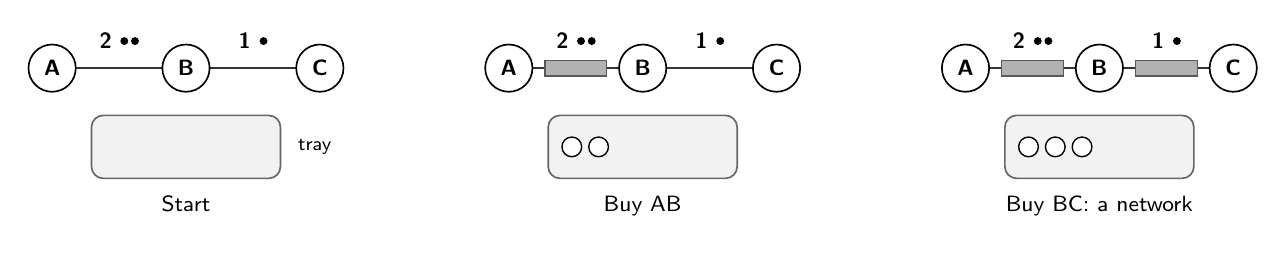
\begin{tikzpicture}[x=1mm,y=1mm]
\draw[line width=0.8pt, black!80] (3.00,15.00) -- (20.00,15.00);
\draw[line width=0.8pt, black!80] (20.00,15.00) -- (37.00,15.00);
\fill[white, rounded corners=0.8mm] (8.35,16.74) rectangle (14.65,20.14);
\node[font=\footnotesize\bfseries, inner sep=0] at (9.80,18.44) {2};
\fill (12.17,18.44) circle (0.5mm);
\fill (13.52,18.44) circle (0.5mm);
\fill[white, rounded corners=0.8mm] (26.02,16.74) rectangle (30.98,20.14);
\node[font=\footnotesize\bfseries, inner sep=0] at (27.47,18.44) {1};
\fill (29.85,18.44) circle (0.5mm);
\node[circle, draw, line width=0.6pt, fill=white, minimum size=6.00mm, inner sep=0, font=\footnotesize\bfseries] at (3.00,15.00) {A};
\node[circle, draw, line width=0.6pt, fill=white, minimum size=6.00mm, inner sep=0, font=\footnotesize\bfseries] at (20.00,15.00) {B};
\node[circle, draw, line width=0.6pt, fill=white, minimum size=6.00mm, inner sep=0, font=\footnotesize\bfseries] at (37.00,15.00) {C};
\draw[black!60, line width=0.6pt, fill=black!5, rounded corners=1.5mm] (8.00,1.00) rectangle (32.00,9.00);
\node[font=\scriptsize, anchor=west] at (33.00,5.00) {tray};
\node[font=\footnotesize, anchor=north, align=center] at (20.00,0.00) {Start};
\draw[line width=0.8pt, black!80] (61.00,15.00) -- (78.00,15.00);
\draw[line width=0.8pt, black!80] (78.00,15.00) -- (95.00,15.00);
\filldraw[fill=black!30, draw=black!65, line width=0.4pt] (65.59,16.00) -- (73.41,16.00) -- (73.41,14.00) -- (65.59,14.00) -- cycle;
\fill[white, rounded corners=0.8mm] (66.35,16.74) rectangle (72.65,20.14);
\node[font=\footnotesize\bfseries, inner sep=0] at (67.80,18.44) {2};
\fill (70.17,18.44) circle (0.5mm);
\fill (71.53,18.44) circle (0.5mm);
\fill[white, rounded corners=0.8mm] (84.03,16.74) rectangle (88.97,20.14);
\node[font=\footnotesize\bfseries, inner sep=0] at (85.48,18.44) {1};
\fill (87.85,18.44) circle (0.5mm);
\node[circle, draw, line width=0.6pt, fill=white, minimum size=6.00mm, inner sep=0, font=\footnotesize\bfseries] at (61.00,15.00) {A};
\node[circle, draw, line width=0.6pt, fill=white, minimum size=6.00mm, inner sep=0, font=\footnotesize\bfseries] at (78.00,15.00) {B};
\node[circle, draw, line width=0.6pt, fill=white, minimum size=6.00mm, inner sep=0, font=\footnotesize\bfseries] at (95.00,15.00) {C};
\draw[black!60, line width=0.6pt, fill=black!5, rounded corners=1.5mm] (66.00,1.00) rectangle (90.00,9.00);
\draw[line width=0.5pt, fill=white] (69.00,5.00) circle (1.25mm);
\draw[line width=0.5pt, fill=white] (72.40,5.00) circle (1.25mm);
\node[font=\footnotesize, anchor=north, align=center] at (78.00,0.00) {Buy AB};
\draw[line width=0.8pt, black!80] (119.00,15.00) -- (136.00,15.00);
\draw[line width=0.8pt, black!80] (136.00,15.00) -- (153.00,15.00);
\filldraw[fill=black!30, draw=black!65, line width=0.4pt] (123.59,16.00) -- (131.41,16.00) -- (131.41,14.00) -- (123.59,14.00) -- cycle;
\filldraw[fill=black!30, draw=black!65, line width=0.4pt] (140.59,16.00) -- (148.41,16.00) -- (148.41,14.00) -- (140.59,14.00) -- cycle;
\fill[white, rounded corners=0.8mm] (124.35,16.74) rectangle (130.65,20.14);
\node[font=\footnotesize\bfseries, inner sep=0] at (125.80,18.44) {2};
\fill (128.18,18.44) circle (0.5mm);
\fill (129.53,18.44) circle (0.5mm);
\fill[white, rounded corners=0.8mm] (142.03,16.74) rectangle (146.97,20.14);
\node[font=\footnotesize\bfseries, inner sep=0] at (143.47,18.44) {1};
\fill (145.85,18.44) circle (0.5mm);
\node[circle, draw, line width=0.6pt, fill=white, minimum size=6.00mm, inner sep=0, font=\footnotesize\bfseries] at (119.00,15.00) {A};
\node[circle, draw, line width=0.6pt, fill=white, minimum size=6.00mm, inner sep=0, font=\footnotesize\bfseries] at (136.00,15.00) {B};
\node[circle, draw, line width=0.6pt, fill=white, minimum size=6.00mm, inner sep=0, font=\footnotesize\bfseries] at (153.00,15.00) {C};
\draw[black!60, line width=0.6pt, fill=black!5, rounded corners=1.5mm] (124.00,1.00) rectangle (148.00,9.00);
\draw[line width=0.5pt, fill=white] (127.00,5.00) circle (1.25mm);
\draw[line width=0.5pt, fill=white] (130.40,5.00) circle (1.25mm);
\draw[line width=0.5pt, fill=white] (133.80,5.00) circle (1.25mm);
\node[font=\footnotesize, anchor=north, align=center] at (136.00,0.00) {Buy BC: a network};
\end{tikzpicture}
\end{center}\par

\vspace{2mm}
\prob{1} Buy a network that costs as few counters as you can. How many different networks cost just that much? Draw each one.

\par\begin{center}
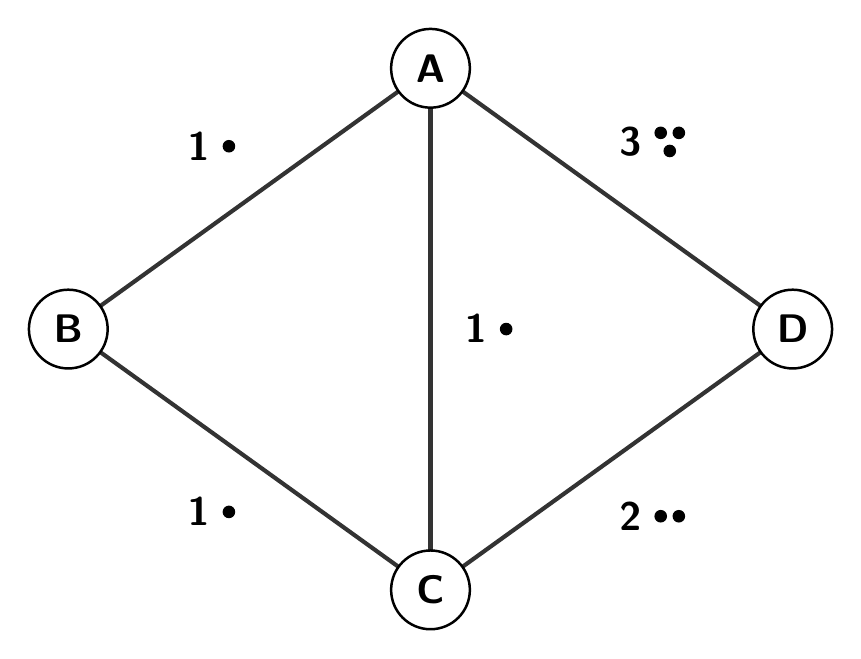
\begin{tikzpicture}[x=1mm,y=1mm]
\draw[line width=1.5pt, black!80] (51.00,71.24) -- (5.00,38.12);
\draw[line width=1.5pt, black!80] (5.00,38.12) -- (51.00,5.00);
\draw[line width=1.5pt, black!80] (51.00,71.24) -- (51.00,5.00);
\draw[line width=1.5pt, black!80] (51.00,5.00) -- (97.00,38.12);
\draw[line width=1.5pt, black!80] (51.00,71.24) -- (97.00,38.12);
\fill[white, rounded corners=0.8mm] (19.25,58.34) rectangle (27.15,64.34);
\node[font=\Large\bfseries, inner sep=0] at (21.55,61.34) {1};
\fill (25.40,61.34) circle (0.8mm);
\fill[white, rounded corners=0.8mm] (19.25,11.90) rectangle (27.15,17.90);
\node[font=\Large\bfseries, inner sep=0] at (21.55,14.90) {1};
\fill (25.40,14.90) circle (0.8mm);
\fill[white, rounded corners=0.8mm] (54.46,35.12) rectangle (62.36,41.12);
\node[font=\Large\bfseries, inner sep=0] at (56.76,38.12) {1};
\fill (60.61,38.12) circle (0.8mm);
\fill[white, rounded corners=0.8mm] (74.09,11.35) rectangle (84.29,17.35);
\node[font=\Large\bfseries, inner sep=0] at (76.39,14.35) {2};
\fill (80.24,14.35) circle (0.8mm);
\fill (82.54,14.35) circle (0.8mm);
\fill[white, rounded corners=0.8mm] (74.09,58.89) rectangle (84.29,64.89);
\node[font=\Large\bfseries, inner sep=0] at (76.39,61.89) {3};
\fill (80.24,63.04) circle (0.8mm);
\fill (82.54,63.04) circle (0.8mm);
\fill (81.39,60.74) circle (0.8mm);
\node[circle, draw, line width=0.9pt, fill=white, minimum size=10.00mm, inner sep=0, font=\Large\bfseries] at (5.00,38.12) {B};
\node[circle, draw, line width=0.9pt, fill=white, minimum size=10.00mm, inner sep=0, font=\Large\bfseries] at (51.00,71.24) {A};
\node[circle, draw, line width=0.9pt, fill=white, minimum size=10.00mm, inner sep=0, font=\Large\bfseries] at (51.00,5.00) {C};
\node[circle, draw, line width=0.9pt, fill=white, minimum size=10.00mm, inner sep=0, font=\Large\bfseries] at (97.00,38.12) {D};
\end{tikzpicture}
\end{center}\par

\vspace{2mm}
\par\begin{center}
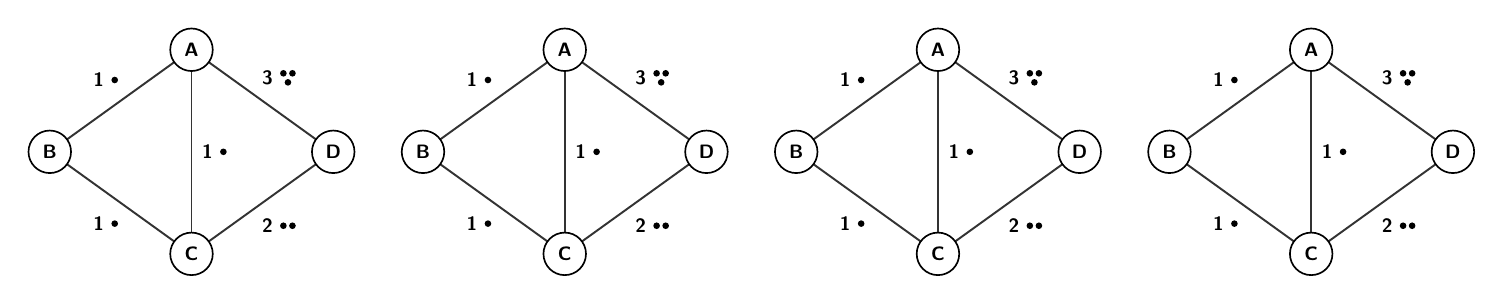
\begin{tikzpicture}[x=1mm,y=1mm]
\draw[line width=0.7pt, black!80] (20.70,28.62) -- (2.70,15.66);
\draw[line width=0.7pt, black!80] (2.70,15.66) -- (20.70,2.70);
\draw[line width=0.7pt, black!80] (20.70,28.62) -- (20.70,2.70);
\draw[line width=0.7pt, black!80] (20.70,2.70) -- (38.70,15.66);
\draw[line width=0.7pt, black!80] (20.70,28.62) -- (38.70,15.66);
\fill[white, rounded corners=0.8mm] (7.72,23.28) rectangle (11.87,26.28);
\node[font=\scriptsize\bfseries, inner sep=0] at (8.92,24.78) {1};
\fill (10.95,24.78) circle (0.42mm);
\fill[white, rounded corners=0.8mm] (7.72,5.04) rectangle (11.87,8.04);
\node[font=\scriptsize\bfseries, inner sep=0] at (8.92,6.54) {1};
\fill (10.95,6.54) circle (0.42mm);
\fill[white, rounded corners=0.8mm] (21.52,14.16) rectangle (25.67,17.16);
\node[font=\scriptsize\bfseries, inner sep=0] at (22.72,15.66) {1};
\fill (24.75,15.66) circle (0.42mm);
\fill[white, rounded corners=0.8mm] (29.15,4.77) rectangle (34.45,7.77);
\node[font=\scriptsize\bfseries, inner sep=0] at (30.35,6.27) {2};
\fill (32.37,6.27) circle (0.42mm);
\fill (33.52,6.27) circle (0.42mm);
\fill[white, rounded corners=0.8mm] (29.15,23.55) rectangle (34.45,26.55);
\node[font=\scriptsize\bfseries, inner sep=0] at (30.35,25.05) {3};
\fill (32.37,25.63) circle (0.42mm);
\fill (33.52,25.63) circle (0.42mm);
\fill (32.95,24.48) circle (0.42mm);
\node[circle, draw, line width=0.6pt, fill=white, minimum size=5.40mm, inner sep=0, font=\scriptsize\bfseries] at (2.70,15.66) {B};
\node[circle, draw, line width=0.6pt, fill=white, minimum size=5.40mm, inner sep=0, font=\scriptsize\bfseries] at (20.70,28.62) {A};
\node[circle, draw, line width=0.6pt, fill=white, minimum size=5.40mm, inner sep=0, font=\scriptsize\bfseries] at (20.70,2.70) {C};
\node[circle, draw, line width=0.6pt, fill=white, minimum size=5.40mm, inner sep=0, font=\scriptsize\bfseries] at (38.70,15.66) {D};
\draw[line width=0.7pt, black!80] (68.10,28.62) -- (50.10,15.66);
\draw[line width=0.7pt, black!80] (50.10,15.66) -- (68.10,2.70);
\draw[line width=0.7pt, black!80] (68.10,28.62) -- (68.10,2.70);
\draw[line width=0.7pt, black!80] (68.10,2.70) -- (86.10,15.66);
\draw[line width=0.7pt, black!80] (68.10,28.62) -- (86.10,15.66);
\fill[white, rounded corners=0.8mm] (55.12,23.28) rectangle (59.27,26.28);
\node[font=\scriptsize\bfseries, inner sep=0] at (56.32,24.78) {1};
\fill (58.35,24.78) circle (0.42mm);
\fill[white, rounded corners=0.8mm] (55.12,5.04) rectangle (59.27,8.04);
\node[font=\scriptsize\bfseries, inner sep=0] at (56.32,6.54) {1};
\fill (58.35,6.54) circle (0.42mm);
\fill[white, rounded corners=0.8mm] (68.92,14.16) rectangle (73.07,17.16);
\node[font=\scriptsize\bfseries, inner sep=0] at (70.12,15.66) {1};
\fill (72.15,15.66) circle (0.42mm);
\fill[white, rounded corners=0.8mm] (76.55,4.77) rectangle (81.85,7.77);
\node[font=\scriptsize\bfseries, inner sep=0] at (77.75,6.27) {2};
\fill (79.77,6.27) circle (0.42mm);
\fill (80.92,6.27) circle (0.42mm);
\fill[white, rounded corners=0.8mm] (76.55,23.55) rectangle (81.85,26.55);
\node[font=\scriptsize\bfseries, inner sep=0] at (77.75,25.05) {3};
\fill (79.77,25.63) circle (0.42mm);
\fill (80.92,25.63) circle (0.42mm);
\fill (80.35,24.48) circle (0.42mm);
\node[circle, draw, line width=0.6pt, fill=white, minimum size=5.40mm, inner sep=0, font=\scriptsize\bfseries] at (50.10,15.66) {B};
\node[circle, draw, line width=0.6pt, fill=white, minimum size=5.40mm, inner sep=0, font=\scriptsize\bfseries] at (68.10,28.62) {A};
\node[circle, draw, line width=0.6pt, fill=white, minimum size=5.40mm, inner sep=0, font=\scriptsize\bfseries] at (68.10,2.70) {C};
\node[circle, draw, line width=0.6pt, fill=white, minimum size=5.40mm, inner sep=0, font=\scriptsize\bfseries] at (86.10,15.66) {D};
\draw[line width=0.7pt, black!80] (115.50,28.62) -- (97.50,15.66);
\draw[line width=0.7pt, black!80] (97.50,15.66) -- (115.50,2.70);
\draw[line width=0.7pt, black!80] (115.50,28.62) -- (115.50,2.70);
\draw[line width=0.7pt, black!80] (115.50,2.70) -- (133.50,15.66);
\draw[line width=0.7pt, black!80] (115.50,28.62) -- (133.50,15.66);
\fill[white, rounded corners=0.8mm] (102.52,23.28) rectangle (106.67,26.28);
\node[font=\scriptsize\bfseries, inner sep=0] at (103.72,24.78) {1};
\fill (105.75,24.78) circle (0.42mm);
\fill[white, rounded corners=0.8mm] (102.52,5.04) rectangle (106.67,8.04);
\node[font=\scriptsize\bfseries, inner sep=0] at (103.72,6.54) {1};
\fill (105.75,6.54) circle (0.42mm);
\fill[white, rounded corners=0.8mm] (116.32,14.16) rectangle (120.47,17.16);
\node[font=\scriptsize\bfseries, inner sep=0] at (117.52,15.66) {1};
\fill (119.55,15.66) circle (0.42mm);
\fill[white, rounded corners=0.8mm] (123.95,4.77) rectangle (129.25,7.77);
\node[font=\scriptsize\bfseries, inner sep=0] at (125.15,6.27) {2};
\fill (127.17,6.27) circle (0.42mm);
\fill (128.32,6.27) circle (0.42mm);
\fill[white, rounded corners=0.8mm] (123.95,23.55) rectangle (129.25,26.55);
\node[font=\scriptsize\bfseries, inner sep=0] at (125.15,25.05) {3};
\fill (127.17,25.63) circle (0.42mm);
\fill (128.32,25.63) circle (0.42mm);
\fill (127.75,24.48) circle (0.42mm);
\node[circle, draw, line width=0.6pt, fill=white, minimum size=5.40mm, inner sep=0, font=\scriptsize\bfseries] at (97.50,15.66) {B};
\node[circle, draw, line width=0.6pt, fill=white, minimum size=5.40mm, inner sep=0, font=\scriptsize\bfseries] at (115.50,28.62) {A};
\node[circle, draw, line width=0.6pt, fill=white, minimum size=5.40mm, inner sep=0, font=\scriptsize\bfseries] at (115.50,2.70) {C};
\node[circle, draw, line width=0.6pt, fill=white, minimum size=5.40mm, inner sep=0, font=\scriptsize\bfseries] at (133.50,15.66) {D};
\draw[line width=0.7pt, black!80] (162.90,28.62) -- (144.90,15.66);
\draw[line width=0.7pt, black!80] (144.90,15.66) -- (162.90,2.70);
\draw[line width=0.7pt, black!80] (162.90,28.62) -- (162.90,2.70);
\draw[line width=0.7pt, black!80] (162.90,2.70) -- (180.90,15.66);
\draw[line width=0.7pt, black!80] (162.90,28.62) -- (180.90,15.66);
\fill[white, rounded corners=0.8mm] (149.92,23.28) rectangle (154.07,26.28);
\node[font=\scriptsize\bfseries, inner sep=0] at (151.12,24.78) {1};
\fill (153.15,24.78) circle (0.42mm);
\fill[white, rounded corners=0.8mm] (149.92,5.04) rectangle (154.07,8.04);
\node[font=\scriptsize\bfseries, inner sep=0] at (151.12,6.54) {1};
\fill (153.15,6.54) circle (0.42mm);
\fill[white, rounded corners=0.8mm] (163.72,14.16) rectangle (167.87,17.16);
\node[font=\scriptsize\bfseries, inner sep=0] at (164.92,15.66) {1};
\fill (166.95,15.66) circle (0.42mm);
\fill[white, rounded corners=0.8mm] (171.35,4.77) rectangle (176.65,7.77);
\node[font=\scriptsize\bfseries, inner sep=0] at (172.55,6.27) {2};
\fill (174.57,6.27) circle (0.42mm);
\fill (175.72,6.27) circle (0.42mm);
\fill[white, rounded corners=0.8mm] (171.35,23.55) rectangle (176.65,26.55);
\node[font=\scriptsize\bfseries, inner sep=0] at (172.55,25.05) {3};
\fill (174.57,25.63) circle (0.42mm);
\fill (175.72,25.63) circle (0.42mm);
\fill (175.15,24.48) circle (0.42mm);
\node[circle, draw, line width=0.6pt, fill=white, minimum size=5.40mm, inner sep=0, font=\scriptsize\bfseries] at (144.90,15.66) {B};
\node[circle, draw, line width=0.6pt, fill=white, minimum size=5.40mm, inner sep=0, font=\scriptsize\bfseries] at (162.90,28.62) {A};
\node[circle, draw, line width=0.6pt, fill=white, minimum size=5.40mm, inner sep=0, font=\scriptsize\bfseries] at (162.90,2.70) {C};
\node[circle, draw, line width=0.6pt, fill=white, minimum size=5.40mm, inner sep=0, font=\scriptsize\bfseries] at (180.90,15.66) {D};
\end{tikzpicture}
\end{center}\par

\newpage

\prob{2} On the big map, lay markers on the 1-dot links, then the 2-dot, 3-dot and 4-dot links, and each time ring the groups of places the pawn can walk between, as in the pictures. When can the pawn first walk from A to F?

\par\begin{center}
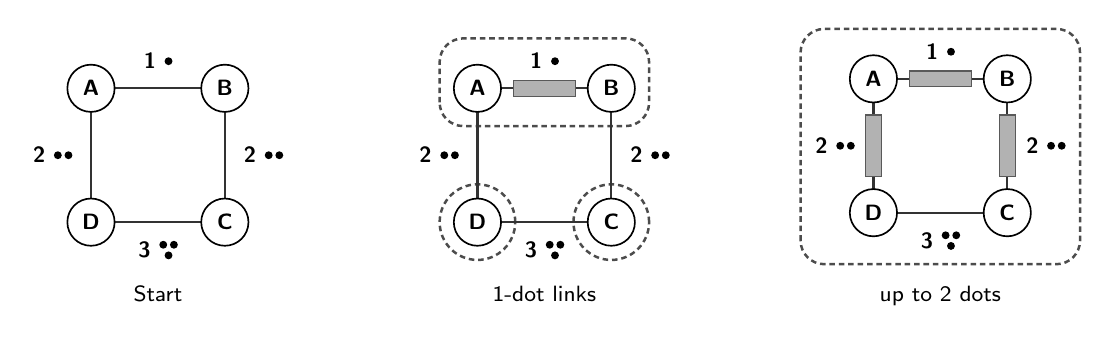
\begin{tikzpicture}[x=1mm,y=1mm]
\draw[line width=0.8pt, black!80] (8.04,27.34) -- (25.04,27.34);
\draw[line width=0.8pt, black!80] (25.04,27.34) -- (25.04,10.34);
\draw[line width=0.8pt, black!80] (25.04,10.34) -- (8.04,10.34);
\draw[line width=0.8pt, black!80] (8.04,10.34) -- (8.04,27.34);
\fill[white, rounded corners=0.8mm] (14.07,29.08) rectangle (19.02,32.48);
\node[font=\footnotesize\bfseries, inner sep=0] at (15.52,30.78) {1};
\fill (17.89,30.78) circle (0.5mm);
\fill[white, rounded corners=0.8mm] (26.78,17.14) rectangle (33.08,20.54);
\node[font=\footnotesize\bfseries, inner sep=0] at (28.23,18.84) {2};
\fill (30.61,18.84) circle (0.5mm);
\fill (31.96,18.84) circle (0.5mm);
\fill[white, rounded corners=0.8mm] (13.39,5.00) rectangle (19.69,8.60);
\node[font=\footnotesize\bfseries, inner sep=0] at (14.84,6.80) {3};
\fill (17.22,7.47) circle (0.5mm);
\fill (18.57,7.47) circle (0.5mm);
\fill (17.89,6.12) circle (0.5mm);
\fill[white, rounded corners=0.8mm] (0.00,17.14) rectangle (6.30,20.54);
\node[font=\footnotesize\bfseries, inner sep=0] at (1.45,18.84) {2};
\fill (3.83,18.84) circle (0.5mm);
\fill (5.18,18.84) circle (0.5mm);
\node[circle, draw, line width=0.6pt, fill=white, minimum size=6.00mm, inner sep=0, font=\footnotesize\bfseries] at (8.04,27.34) {A};
\node[circle, draw, line width=0.6pt, fill=white, minimum size=6.00mm, inner sep=0, font=\footnotesize\bfseries] at (25.04,27.34) {B};
\node[circle, draw, line width=0.6pt, fill=white, minimum size=6.00mm, inner sep=0, font=\footnotesize\bfseries] at (25.04,10.34) {C};
\node[circle, draw, line width=0.6pt, fill=white, minimum size=6.00mm, inner sep=0, font=\footnotesize\bfseries] at (8.04,10.34) {D};
\node[font=\footnotesize, anchor=north, align=center] at (16.54,3.50) {Start};
\draw[black!70, line width=0.9pt, dash pattern=on 2pt off 1.4pt, rounded corners=3mm] (52.32,22.54) rectangle (78.92,33.68);
\draw[black!70, line width=0.9pt, dash pattern=on 2pt off 1.4pt] (74.12,10.34) circle (4.80mm);
\draw[black!70, line width=0.9pt, dash pattern=on 2pt off 1.4pt] (57.12,10.34) circle (4.80mm);
\draw[line width=0.8pt, black!80] (57.12,27.34) -- (74.12,27.34);
\draw[line width=0.8pt, black!80] (74.12,27.34) -- (74.12,10.34);
\draw[line width=0.8pt, black!80] (74.12,10.34) -- (57.12,10.34);
\draw[line width=0.8pt, black!80] (57.12,10.34) -- (57.12,27.34);
\filldraw[fill=black!30, draw=black!65, line width=0.4pt] (61.71,28.34) -- (69.53,28.34) -- (69.53,26.34) -- (61.71,26.34) -- cycle;
\fill[white, rounded corners=0.8mm] (63.15,29.08) rectangle (68.10,32.48);
\node[font=\footnotesize\bfseries, inner sep=0] at (64.60,30.78) {1};
\fill (66.97,30.78) circle (0.5mm);
\fill[white, rounded corners=0.8mm] (75.86,17.14) rectangle (82.16,20.54);
\node[font=\footnotesize\bfseries, inner sep=0] at (77.31,18.84) {2};
\fill (79.69,18.84) circle (0.5mm);
\fill (81.04,18.84) circle (0.5mm);
\fill[white, rounded corners=0.8mm] (62.47,5.00) rectangle (68.77,8.60);
\node[font=\footnotesize\bfseries, inner sep=0] at (63.92,6.80) {3};
\fill (66.30,7.47) circle (0.5mm);
\fill (67.65,7.47) circle (0.5mm);
\fill (66.97,6.12) circle (0.5mm);
\fill[white, rounded corners=0.8mm] (49.08,17.14) rectangle (55.38,20.54);
\node[font=\footnotesize\bfseries, inner sep=0] at (50.53,18.84) {2};
\fill (52.91,18.84) circle (0.5mm);
\fill (54.26,18.84) circle (0.5mm);
\node[circle, draw, line width=0.6pt, fill=white, minimum size=6.00mm, inner sep=0, font=\footnotesize\bfseries] at (57.12,27.34) {A};
\node[circle, draw, line width=0.6pt, fill=white, minimum size=6.00mm, inner sep=0, font=\footnotesize\bfseries] at (74.12,27.34) {B};
\node[circle, draw, line width=0.6pt, fill=white, minimum size=6.00mm, inner sep=0, font=\footnotesize\bfseries] at (74.12,10.34) {C};
\node[circle, draw, line width=0.6pt, fill=white, minimum size=6.00mm, inner sep=0, font=\footnotesize\bfseries] at (57.12,10.34) {D};
\node[font=\footnotesize, anchor=north, align=center] at (65.62,3.50) {1-dot links};
\draw[black!70, line width=0.9pt, dash pattern=on 2pt off 1.4pt, rounded corners=3mm] (98.16,5.00) rectangle (133.65,34.88);
\draw[line width=0.8pt, black!80] (107.41,28.54) -- (124.41,28.54);
\draw[line width=0.8pt, black!80] (124.41,28.54) -- (124.41,11.54);
\draw[line width=0.8pt, black!80] (124.41,11.54) -- (107.41,11.54);
\draw[line width=0.8pt, black!80] (107.41,11.54) -- (107.41,28.54);
\filldraw[fill=black!30, draw=black!65, line width=0.4pt] (112.00,29.54) -- (119.82,29.54) -- (119.82,27.54) -- (112.00,27.54) -- cycle;
\filldraw[fill=black!30, draw=black!65, line width=0.4pt] (125.41,23.95) -- (125.41,16.13) -- (123.41,16.13) -- (123.41,23.95) -- cycle;
\filldraw[fill=black!30, draw=black!65, line width=0.4pt] (106.41,16.13) -- (106.41,23.95) -- (108.41,23.95) -- (108.41,16.13) -- cycle;
\fill[white, rounded corners=0.8mm] (113.43,30.28) rectangle (118.38,33.68);
\node[font=\footnotesize\bfseries, inner sep=0] at (114.88,31.98) {1};
\fill (117.26,31.98) circle (0.5mm);
\fill[white, rounded corners=0.8mm] (126.15,18.34) rectangle (132.45,21.74);
\node[font=\footnotesize\bfseries, inner sep=0] at (127.60,20.04) {2};
\fill (129.97,20.04) circle (0.5mm);
\fill (131.32,20.04) circle (0.5mm);
\fill[white, rounded corners=0.8mm] (112.76,6.20) rectangle (119.06,9.80);
\node[font=\footnotesize\bfseries, inner sep=0] at (114.21,8.00) {3};
\fill (116.58,8.67) circle (0.5mm);
\fill (117.93,8.67) circle (0.5mm);
\fill (117.26,7.32) circle (0.5mm);
\fill[white, rounded corners=0.8mm] (99.36,18.34) rectangle (105.66,21.74);
\node[font=\footnotesize\bfseries, inner sep=0] at (100.81,20.04) {2};
\fill (103.19,20.04) circle (0.5mm);
\fill (104.54,20.04) circle (0.5mm);
\node[circle, draw, line width=0.6pt, fill=white, minimum size=6.00mm, inner sep=0, font=\footnotesize\bfseries] at (107.41,28.54) {A};
\node[circle, draw, line width=0.6pt, fill=white, minimum size=6.00mm, inner sep=0, font=\footnotesize\bfseries] at (124.41,28.54) {B};
\node[circle, draw, line width=0.6pt, fill=white, minimum size=6.00mm, inner sep=0, font=\footnotesize\bfseries] at (124.41,11.54) {C};
\node[circle, draw, line width=0.6pt, fill=white, minimum size=6.00mm, inner sep=0, font=\footnotesize\bfseries] at (107.41,11.54) {D};
\node[font=\footnotesize, anchor=north, align=center] at (115.91,3.50) {up to 2 dots};
\end{tikzpicture}
\end{center}\par

\par\begin{center}
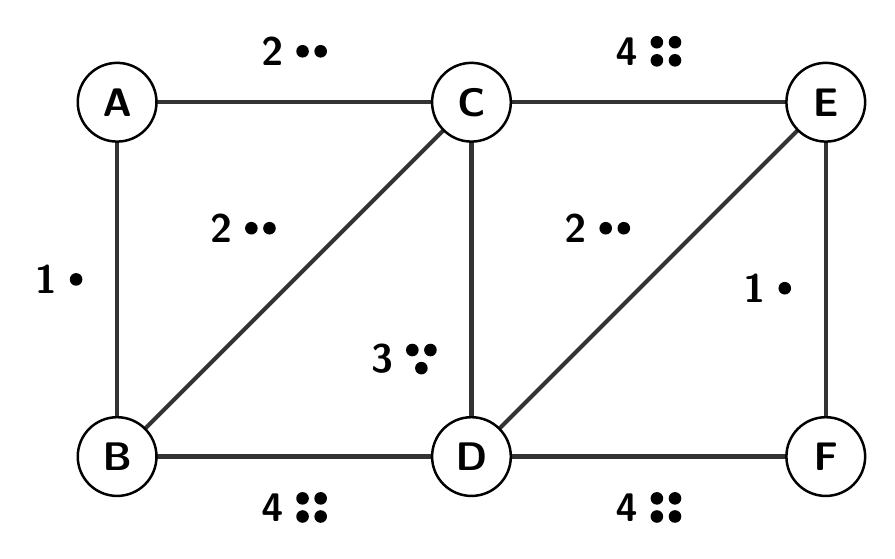
\begin{tikzpicture}[x=1mm,y=1mm]
\draw[line width=1.5pt, black!80] (11.36,54.46) -- (11.36,9.46);
\draw[line width=1.5pt, black!80] (11.36,54.46) -- (56.36,54.46);
\draw[line width=1.5pt, black!80] (11.36,9.46) -- (56.36,54.46);
\draw[line width=1.5pt, black!80] (56.36,54.46) -- (56.36,9.46);
\draw[line width=1.5pt, black!80] (11.36,9.46) -- (56.36,9.46);
\draw[line width=1.5pt, black!80] (56.36,54.46) -- (101.36,54.46);
\draw[line width=1.5pt, black!80] (56.36,9.46) -- (101.36,54.46);
\draw[line width=1.5pt, black!80] (101.36,54.46) -- (101.36,9.46);
\draw[line width=1.5pt, black!80] (56.36,9.46) -- (101.36,9.46);
\fill[white, rounded corners=0.8mm] (-0.00,28.96) rectangle (7.90,34.96);
\node[font=\Large\bfseries, inner sep=0] at (2.30,31.96) {1};
\fill (6.15,31.96) circle (0.8mm);
\fill[white, rounded corners=0.8mm] (28.76,57.93) rectangle (38.96,63.93);
\node[font=\Large\bfseries, inner sep=0] at (31.06,60.93) {2};
\fill (34.91,60.93) circle (0.8mm);
\fill (37.21,60.93) circle (0.8mm);
\fill[white, rounded corners=0.8mm] (22.26,35.46) rectangle (32.46,41.46);
\node[font=\Large\bfseries, inner sep=0] at (24.56,38.46) {2};
\fill (28.41,38.46) circle (0.8mm);
\fill (30.71,38.46) circle (0.8mm);
\fill[white, rounded corners=0.8mm] (42.70,18.84) rectangle (52.90,24.84);
\node[font=\Large\bfseries, inner sep=0] at (45.00,21.84) {3};
\fill (48.85,22.99) circle (0.8mm);
\fill (51.15,22.99) circle (0.8mm);
\fill (50.00,20.69) circle (0.8mm);
\fill[white, rounded corners=0.8mm] (28.76,0.00) rectangle (38.96,6.00);
\node[font=\Large\bfseries, inner sep=0] at (31.06,3.00) {4};
\fill (34.91,4.15) circle (0.8mm);
\fill (37.21,4.15) circle (0.8mm);
\fill (34.91,1.85) circle (0.8mm);
\fill (37.21,1.85) circle (0.8mm);
\fill[white, rounded corners=0.8mm] (73.76,57.93) rectangle (83.96,63.93);
\node[font=\Large\bfseries, inner sep=0] at (76.06,60.93) {4};
\fill (79.91,62.08) circle (0.8mm);
\fill (82.21,62.08) circle (0.8mm);
\fill (79.91,59.78) circle (0.8mm);
\fill (82.21,59.78) circle (0.8mm);
\fill[white, rounded corners=0.8mm] (67.26,35.46) rectangle (77.46,41.46);
\node[font=\Large\bfseries, inner sep=0] at (69.56,38.46) {2};
\fill (73.41,38.46) circle (0.8mm);
\fill (75.71,38.46) circle (0.8mm);
\fill[white, rounded corners=0.8mm] (90.00,27.84) rectangle (97.90,33.84);
\node[font=\Large\bfseries, inner sep=0] at (92.30,30.84) {1};
\fill (96.15,30.84) circle (0.8mm);
\fill[white, rounded corners=0.8mm] (73.76,0.00) rectangle (83.96,6.00);
\node[font=\Large\bfseries, inner sep=0] at (76.06,3.00) {4};
\fill (79.91,4.15) circle (0.8mm);
\fill (82.21,4.15) circle (0.8mm);
\fill (79.91,1.85) circle (0.8mm);
\fill (82.21,1.85) circle (0.8mm);
\node[circle, draw, line width=0.9pt, fill=white, minimum size=10.00mm, inner sep=0, font=\Large\bfseries] at (11.36,54.46) {A};
\node[circle, draw, line width=0.9pt, fill=white, minimum size=10.00mm, inner sep=0, font=\Large\bfseries] at (56.36,54.46) {C};
\node[circle, draw, line width=0.9pt, fill=white, minimum size=10.00mm, inner sep=0, font=\Large\bfseries] at (101.36,54.46) {E};
\node[circle, draw, line width=0.9pt, fill=white, minimum size=10.00mm, inner sep=0, font=\Large\bfseries] at (11.36,9.46) {B};
\node[circle, draw, line width=0.9pt, fill=white, minimum size=10.00mm, inner sep=0, font=\Large\bfseries] at (56.36,9.46) {D};
\node[circle, draw, line width=0.9pt, fill=white, minimum size=10.00mm, inner sep=0, font=\Large\bfseries] at (101.36,9.46) {F};
\end{tikzpicture}
\end{center}\par

\vspace{1mm}
\par\begin{center}
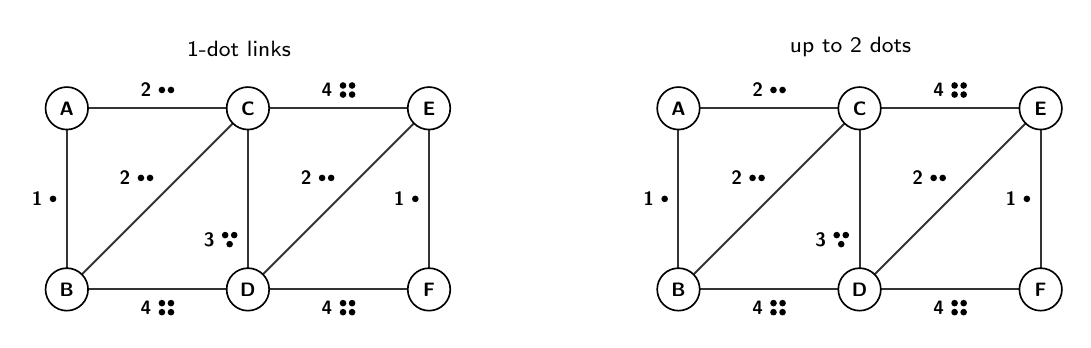
\begin{tikzpicture}[x=1mm,y=1mm]
\draw[line width=0.7pt, black!80] (4.97,26.82) -- (4.97,3.82);
\draw[line width=0.7pt, black!80] (4.97,26.82) -- (27.97,26.82);
\draw[line width=0.7pt, black!80] (4.97,3.82) -- (27.97,26.82);
\draw[line width=0.7pt, black!80] (27.97,26.82) -- (27.97,3.82);
\draw[line width=0.7pt, black!80] (4.97,3.82) -- (27.97,3.82);
\draw[line width=0.7pt, black!80] (27.97,26.82) -- (50.97,26.82);
\draw[line width=0.7pt, black!80] (27.97,3.82) -- (50.97,26.82);
\draw[line width=0.7pt, black!80] (50.97,26.82) -- (50.97,3.82);
\draw[line width=0.7pt, black!80] (27.97,3.82) -- (50.97,3.82);
\fill[white, rounded corners=0.8mm] (0.00,13.82) rectangle (4.15,16.82);
\node[font=\scriptsize\bfseries, inner sep=0] at (1.20,15.32) {1};
\fill (3.22,15.32) circle (0.42mm);
\fill[white, rounded corners=0.8mm] (13.82,27.65) rectangle (19.12,30.65);
\node[font=\scriptsize\bfseries, inner sep=0] at (15.02,29.15) {2};
\fill (17.05,29.15) circle (0.42mm);
\fill (18.20,29.15) circle (0.42mm);
\fill[white, rounded corners=0.8mm] (11.17,16.48) rectangle (16.47,19.48);
\node[font=\scriptsize\bfseries, inner sep=0] at (12.37,17.98) {2};
\fill (14.39,17.98) circle (0.42mm);
\fill (15.54,17.98) circle (0.42mm);
\fill[white, rounded corners=0.8mm] (21.85,8.65) rectangle (27.15,11.65);
\node[font=\scriptsize\bfseries, inner sep=0] at (23.05,10.15) {3};
\fill (25.08,10.72) circle (0.42mm);
\fill (26.23,10.72) circle (0.42mm);
\fill (25.65,9.57) circle (0.42mm);
\fill[white, rounded corners=0.8mm] (13.82,0.00) rectangle (19.12,3.00);
\node[font=\scriptsize\bfseries, inner sep=0] at (15.02,1.50) {4};
\fill (17.05,2.08) circle (0.42mm);
\fill (18.20,2.08) circle (0.42mm);
\fill (17.05,0.93) circle (0.42mm);
\fill (18.20,0.93) circle (0.42mm);
\fill[white, rounded corners=0.8mm] (36.82,27.65) rectangle (42.12,30.65);
\node[font=\scriptsize\bfseries, inner sep=0] at (38.02,29.15) {4};
\fill (40.05,29.72) circle (0.42mm);
\fill (41.20,29.72) circle (0.42mm);
\fill (40.05,28.57) circle (0.42mm);
\fill (41.20,28.57) circle (0.42mm);
\fill[white, rounded corners=0.8mm] (34.17,16.48) rectangle (39.47,19.48);
\node[font=\scriptsize\bfseries, inner sep=0] at (35.37,17.98) {2};
\fill (37.39,17.98) circle (0.42mm);
\fill (38.54,17.98) circle (0.42mm);
\fill[white, rounded corners=0.8mm] (46.00,13.82) rectangle (50.15,16.82);
\node[font=\scriptsize\bfseries, inner sep=0] at (47.20,15.32) {1};
\fill (49.23,15.32) circle (0.42mm);
\fill[white, rounded corners=0.8mm] (36.82,0.00) rectangle (42.12,3.00);
\node[font=\scriptsize\bfseries, inner sep=0] at (38.02,1.50) {4};
\fill (40.05,2.08) circle (0.42mm);
\fill (41.20,2.08) circle (0.42mm);
\fill (40.05,0.93) circle (0.42mm);
\fill (41.20,0.93) circle (0.42mm);
\node[circle, draw, line width=0.6pt, fill=white, minimum size=5.40mm, inner sep=0, font=\scriptsize\bfseries] at (4.97,26.82) {A};
\node[circle, draw, line width=0.6pt, fill=white, minimum size=5.40mm, inner sep=0, font=\scriptsize\bfseries] at (27.97,26.82) {C};
\node[circle, draw, line width=0.6pt, fill=white, minimum size=5.40mm, inner sep=0, font=\scriptsize\bfseries] at (50.97,26.82) {E};
\node[circle, draw, line width=0.6pt, fill=white, minimum size=5.40mm, inner sep=0, font=\scriptsize\bfseries] at (4.97,3.82) {B};
\node[circle, draw, line width=0.6pt, fill=white, minimum size=5.40mm, inner sep=0, font=\scriptsize\bfseries] at (27.97,3.82) {D};
\node[circle, draw, line width=0.6pt, fill=white, minimum size=5.40mm, inner sep=0, font=\scriptsize\bfseries] at (50.97,3.82) {F};
\node[font=\footnotesize, anchor=south, align=center] at (26.84,32.15) {1-dot links};
\draw[line width=0.7pt, black!80] (82.65,26.82) -- (82.65,3.82);
\draw[line width=0.7pt, black!80] (82.65,26.82) -- (105.65,26.82);
\draw[line width=0.7pt, black!80] (82.65,3.82) -- (105.65,26.82);
\draw[line width=0.7pt, black!80] (105.65,26.82) -- (105.65,3.82);
\draw[line width=0.7pt, black!80] (82.65,3.82) -- (105.65,3.82);
\draw[line width=0.7pt, black!80] (105.65,26.82) -- (128.65,26.82);
\draw[line width=0.7pt, black!80] (105.65,3.82) -- (128.65,26.82);
\draw[line width=0.7pt, black!80] (128.65,26.82) -- (128.65,3.82);
\draw[line width=0.7pt, black!80] (105.65,3.82) -- (128.65,3.82);
\fill[white, rounded corners=0.8mm] (77.67,13.82) rectangle (81.82,16.82);
\node[font=\scriptsize\bfseries, inner sep=0] at (78.87,15.32) {1};
\fill (80.90,15.32) circle (0.42mm);
\fill[white, rounded corners=0.8mm] (91.50,27.65) rectangle (96.80,30.65);
\node[font=\scriptsize\bfseries, inner sep=0] at (92.70,29.15) {2};
\fill (94.72,29.15) circle (0.42mm);
\fill (95.87,29.15) circle (0.42mm);
\fill[white, rounded corners=0.8mm] (88.84,16.48) rectangle (94.14,19.48);
\node[font=\scriptsize\bfseries, inner sep=0] at (90.04,17.98) {2};
\fill (92.06,17.98) circle (0.42mm);
\fill (93.21,17.98) circle (0.42mm);
\fill[white, rounded corners=0.8mm] (99.52,8.65) rectangle (104.82,11.65);
\node[font=\scriptsize\bfseries, inner sep=0] at (100.72,10.15) {3};
\fill (102.75,10.72) circle (0.42mm);
\fill (103.90,10.72) circle (0.42mm);
\fill (103.32,9.57) circle (0.42mm);
\fill[white, rounded corners=0.8mm] (91.50,0.00) rectangle (96.80,3.00);
\node[font=\scriptsize\bfseries, inner sep=0] at (92.70,1.50) {4};
\fill (94.72,2.08) circle (0.42mm);
\fill (95.87,2.08) circle (0.42mm);
\fill (94.72,0.93) circle (0.42mm);
\fill (95.87,0.93) circle (0.42mm);
\fill[white, rounded corners=0.8mm] (114.50,27.65) rectangle (119.80,30.65);
\node[font=\scriptsize\bfseries, inner sep=0] at (115.70,29.15) {4};
\fill (117.72,29.72) circle (0.42mm);
\fill (118.87,29.72) circle (0.42mm);
\fill (117.72,28.57) circle (0.42mm);
\fill (118.87,28.57) circle (0.42mm);
\fill[white, rounded corners=0.8mm] (111.84,16.48) rectangle (117.14,19.48);
\node[font=\scriptsize\bfseries, inner sep=0] at (113.04,17.98) {2};
\fill (115.06,17.98) circle (0.42mm);
\fill (116.21,17.98) circle (0.42mm);
\fill[white, rounded corners=0.8mm] (123.67,13.82) rectangle (127.82,16.82);
\node[font=\scriptsize\bfseries, inner sep=0] at (124.87,15.32) {1};
\fill (126.90,15.32) circle (0.42mm);
\fill[white, rounded corners=0.8mm] (114.50,0.00) rectangle (119.80,3.00);
\node[font=\scriptsize\bfseries, inner sep=0] at (115.70,1.50) {4};
\fill (117.72,2.08) circle (0.42mm);
\fill (118.87,2.08) circle (0.42mm);
\fill (117.72,0.93) circle (0.42mm);
\fill (118.87,0.93) circle (0.42mm);
\node[circle, draw, line width=0.6pt, fill=white, minimum size=5.40mm, inner sep=0, font=\scriptsize\bfseries] at (82.65,26.82) {A};
\node[circle, draw, line width=0.6pt, fill=white, minimum size=5.40mm, inner sep=0, font=\scriptsize\bfseries] at (105.65,26.82) {C};
\node[circle, draw, line width=0.6pt, fill=white, minimum size=5.40mm, inner sep=0, font=\scriptsize\bfseries] at (128.65,26.82) {E};
\node[circle, draw, line width=0.6pt, fill=white, minimum size=5.40mm, inner sep=0, font=\scriptsize\bfseries] at (82.65,3.82) {B};
\node[circle, draw, line width=0.6pt, fill=white, minimum size=5.40mm, inner sep=0, font=\scriptsize\bfseries] at (105.65,3.82) {D};
\node[circle, draw, line width=0.6pt, fill=white, minimum size=5.40mm, inner sep=0, font=\scriptsize\bfseries] at (128.65,3.82) {F};
\node[font=\footnotesize, anchor=south, align=center] at (104.51,32.15) {up to 2 dots};
\end{tikzpicture}
\end{center}\par

\par\begin{center}
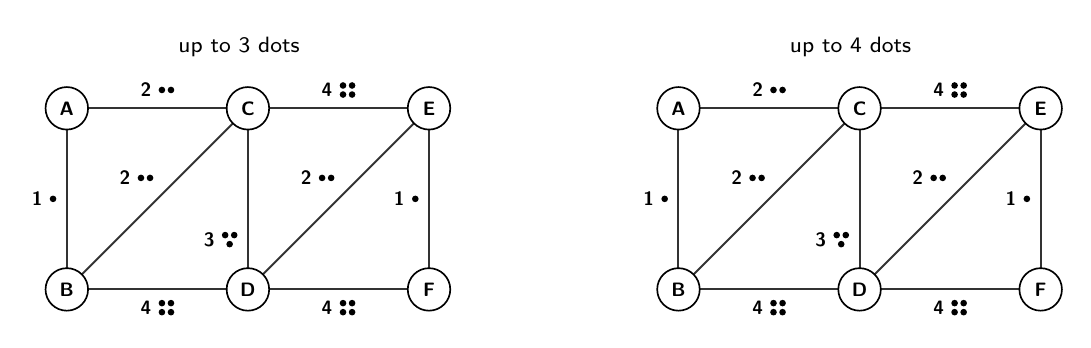
\begin{tikzpicture}[x=1mm,y=1mm]
\draw[line width=0.7pt, black!80] (4.97,26.82) -- (4.97,3.82);
\draw[line width=0.7pt, black!80] (4.97,26.82) -- (27.97,26.82);
\draw[line width=0.7pt, black!80] (4.97,3.82) -- (27.97,26.82);
\draw[line width=0.7pt, black!80] (27.97,26.82) -- (27.97,3.82);
\draw[line width=0.7pt, black!80] (4.97,3.82) -- (27.97,3.82);
\draw[line width=0.7pt, black!80] (27.97,26.82) -- (50.97,26.82);
\draw[line width=0.7pt, black!80] (27.97,3.82) -- (50.97,26.82);
\draw[line width=0.7pt, black!80] (50.97,26.82) -- (50.97,3.82);
\draw[line width=0.7pt, black!80] (27.97,3.82) -- (50.97,3.82);
\fill[white, rounded corners=0.8mm] (0.00,13.82) rectangle (4.15,16.82);
\node[font=\scriptsize\bfseries, inner sep=0] at (1.20,15.32) {1};
\fill (3.22,15.32) circle (0.42mm);
\fill[white, rounded corners=0.8mm] (13.82,27.65) rectangle (19.12,30.65);
\node[font=\scriptsize\bfseries, inner sep=0] at (15.02,29.15) {2};
\fill (17.05,29.15) circle (0.42mm);
\fill (18.20,29.15) circle (0.42mm);
\fill[white, rounded corners=0.8mm] (11.17,16.48) rectangle (16.47,19.48);
\node[font=\scriptsize\bfseries, inner sep=0] at (12.37,17.98) {2};
\fill (14.39,17.98) circle (0.42mm);
\fill (15.54,17.98) circle (0.42mm);
\fill[white, rounded corners=0.8mm] (21.85,8.65) rectangle (27.15,11.65);
\node[font=\scriptsize\bfseries, inner sep=0] at (23.05,10.15) {3};
\fill (25.08,10.72) circle (0.42mm);
\fill (26.23,10.72) circle (0.42mm);
\fill (25.65,9.57) circle (0.42mm);
\fill[white, rounded corners=0.8mm] (13.82,0.00) rectangle (19.12,3.00);
\node[font=\scriptsize\bfseries, inner sep=0] at (15.02,1.50) {4};
\fill (17.05,2.08) circle (0.42mm);
\fill (18.20,2.08) circle (0.42mm);
\fill (17.05,0.93) circle (0.42mm);
\fill (18.20,0.93) circle (0.42mm);
\fill[white, rounded corners=0.8mm] (36.82,27.65) rectangle (42.12,30.65);
\node[font=\scriptsize\bfseries, inner sep=0] at (38.02,29.15) {4};
\fill (40.05,29.72) circle (0.42mm);
\fill (41.20,29.72) circle (0.42mm);
\fill (40.05,28.57) circle (0.42mm);
\fill (41.20,28.57) circle (0.42mm);
\fill[white, rounded corners=0.8mm] (34.17,16.48) rectangle (39.47,19.48);
\node[font=\scriptsize\bfseries, inner sep=0] at (35.37,17.98) {2};
\fill (37.39,17.98) circle (0.42mm);
\fill (38.54,17.98) circle (0.42mm);
\fill[white, rounded corners=0.8mm] (46.00,13.82) rectangle (50.15,16.82);
\node[font=\scriptsize\bfseries, inner sep=0] at (47.20,15.32) {1};
\fill (49.23,15.32) circle (0.42mm);
\fill[white, rounded corners=0.8mm] (36.82,0.00) rectangle (42.12,3.00);
\node[font=\scriptsize\bfseries, inner sep=0] at (38.02,1.50) {4};
\fill (40.05,2.08) circle (0.42mm);
\fill (41.20,2.08) circle (0.42mm);
\fill (40.05,0.93) circle (0.42mm);
\fill (41.20,0.93) circle (0.42mm);
\node[circle, draw, line width=0.6pt, fill=white, minimum size=5.40mm, inner sep=0, font=\scriptsize\bfseries] at (4.97,26.82) {A};
\node[circle, draw, line width=0.6pt, fill=white, minimum size=5.40mm, inner sep=0, font=\scriptsize\bfseries] at (27.97,26.82) {C};
\node[circle, draw, line width=0.6pt, fill=white, minimum size=5.40mm, inner sep=0, font=\scriptsize\bfseries] at (50.97,26.82) {E};
\node[circle, draw, line width=0.6pt, fill=white, minimum size=5.40mm, inner sep=0, font=\scriptsize\bfseries] at (4.97,3.82) {B};
\node[circle, draw, line width=0.6pt, fill=white, minimum size=5.40mm, inner sep=0, font=\scriptsize\bfseries] at (27.97,3.82) {D};
\node[circle, draw, line width=0.6pt, fill=white, minimum size=5.40mm, inner sep=0, font=\scriptsize\bfseries] at (50.97,3.82) {F};
\node[font=\footnotesize, anchor=south, align=center] at (26.84,32.15) {up to 3 dots};
\draw[line width=0.7pt, black!80] (82.65,26.82) -- (82.65,3.82);
\draw[line width=0.7pt, black!80] (82.65,26.82) -- (105.65,26.82);
\draw[line width=0.7pt, black!80] (82.65,3.82) -- (105.65,26.82);
\draw[line width=0.7pt, black!80] (105.65,26.82) -- (105.65,3.82);
\draw[line width=0.7pt, black!80] (82.65,3.82) -- (105.65,3.82);
\draw[line width=0.7pt, black!80] (105.65,26.82) -- (128.65,26.82);
\draw[line width=0.7pt, black!80] (105.65,3.82) -- (128.65,26.82);
\draw[line width=0.7pt, black!80] (128.65,26.82) -- (128.65,3.82);
\draw[line width=0.7pt, black!80] (105.65,3.82) -- (128.65,3.82);
\fill[white, rounded corners=0.8mm] (77.67,13.82) rectangle (81.82,16.82);
\node[font=\scriptsize\bfseries, inner sep=0] at (78.87,15.32) {1};
\fill (80.90,15.32) circle (0.42mm);
\fill[white, rounded corners=0.8mm] (91.50,27.65) rectangle (96.80,30.65);
\node[font=\scriptsize\bfseries, inner sep=0] at (92.70,29.15) {2};
\fill (94.72,29.15) circle (0.42mm);
\fill (95.87,29.15) circle (0.42mm);
\fill[white, rounded corners=0.8mm] (88.84,16.48) rectangle (94.14,19.48);
\node[font=\scriptsize\bfseries, inner sep=0] at (90.04,17.98) {2};
\fill (92.06,17.98) circle (0.42mm);
\fill (93.21,17.98) circle (0.42mm);
\fill[white, rounded corners=0.8mm] (99.52,8.65) rectangle (104.82,11.65);
\node[font=\scriptsize\bfseries, inner sep=0] at (100.72,10.15) {3};
\fill (102.75,10.72) circle (0.42mm);
\fill (103.90,10.72) circle (0.42mm);
\fill (103.32,9.57) circle (0.42mm);
\fill[white, rounded corners=0.8mm] (91.50,0.00) rectangle (96.80,3.00);
\node[font=\scriptsize\bfseries, inner sep=0] at (92.70,1.50) {4};
\fill (94.72,2.08) circle (0.42mm);
\fill (95.87,2.08) circle (0.42mm);
\fill (94.72,0.93) circle (0.42mm);
\fill (95.87,0.93) circle (0.42mm);
\fill[white, rounded corners=0.8mm] (114.50,27.65) rectangle (119.80,30.65);
\node[font=\scriptsize\bfseries, inner sep=0] at (115.70,29.15) {4};
\fill (117.72,29.72) circle (0.42mm);
\fill (118.87,29.72) circle (0.42mm);
\fill (117.72,28.57) circle (0.42mm);
\fill (118.87,28.57) circle (0.42mm);
\fill[white, rounded corners=0.8mm] (111.84,16.48) rectangle (117.14,19.48);
\node[font=\scriptsize\bfseries, inner sep=0] at (113.04,17.98) {2};
\fill (115.06,17.98) circle (0.42mm);
\fill (116.21,17.98) circle (0.42mm);
\fill[white, rounded corners=0.8mm] (123.67,13.82) rectangle (127.82,16.82);
\node[font=\scriptsize\bfseries, inner sep=0] at (124.87,15.32) {1};
\fill (126.90,15.32) circle (0.42mm);
\fill[white, rounded corners=0.8mm] (114.50,0.00) rectangle (119.80,3.00);
\node[font=\scriptsize\bfseries, inner sep=0] at (115.70,1.50) {4};
\fill (117.72,2.08) circle (0.42mm);
\fill (118.87,2.08) circle (0.42mm);
\fill (117.72,0.93) circle (0.42mm);
\fill (118.87,0.93) circle (0.42mm);
\node[circle, draw, line width=0.6pt, fill=white, minimum size=5.40mm, inner sep=0, font=\scriptsize\bfseries] at (82.65,26.82) {A};
\node[circle, draw, line width=0.6pt, fill=white, minimum size=5.40mm, inner sep=0, font=\scriptsize\bfseries] at (105.65,26.82) {C};
\node[circle, draw, line width=0.6pt, fill=white, minimum size=5.40mm, inner sep=0, font=\scriptsize\bfseries] at (128.65,26.82) {E};
\node[circle, draw, line width=0.6pt, fill=white, minimum size=5.40mm, inner sep=0, font=\scriptsize\bfseries] at (82.65,3.82) {B};
\node[circle, draw, line width=0.6pt, fill=white, minimum size=5.40mm, inner sep=0, font=\scriptsize\bfseries] at (105.65,3.82) {D};
\node[circle, draw, line width=0.6pt, fill=white, minimum size=5.40mm, inner sep=0, font=\scriptsize\bfseries] at (128.65,3.82) {F};
\node[font=\footnotesize, anchor=south, align=center] at (104.51,32.15) {up to 4 dots};
\end{tikzpicture}
\end{center}\par

\newpage

\prob{3} Buy the cheapest network you can on this map. Can you buy a network that has no link with 3 or 4 dots?

\par\begin{center}
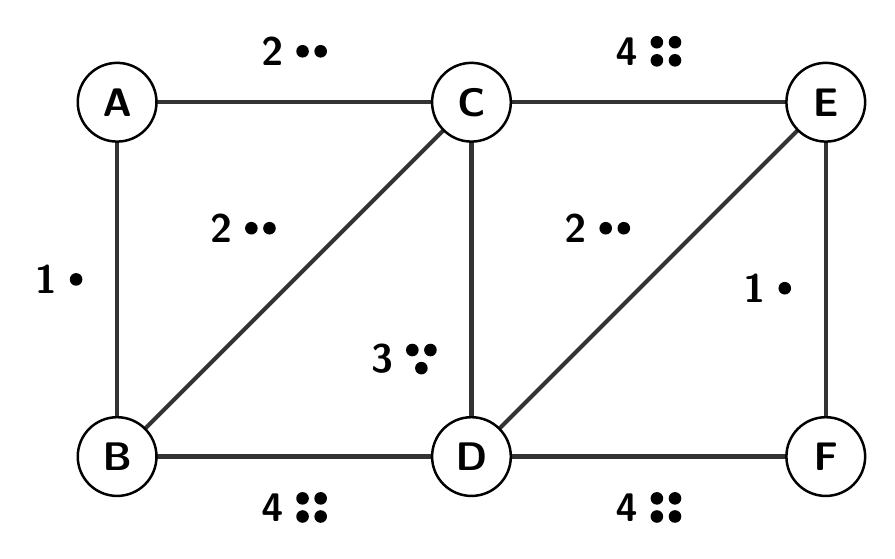
\begin{tikzpicture}[x=1mm,y=1mm]
\draw[line width=1.5pt, black!80] (11.36,54.46) -- (11.36,9.46);
\draw[line width=1.5pt, black!80] (11.36,54.46) -- (56.36,54.46);
\draw[line width=1.5pt, black!80] (11.36,9.46) -- (56.36,54.46);
\draw[line width=1.5pt, black!80] (56.36,54.46) -- (56.36,9.46);
\draw[line width=1.5pt, black!80] (11.36,9.46) -- (56.36,9.46);
\draw[line width=1.5pt, black!80] (56.36,54.46) -- (101.36,54.46);
\draw[line width=1.5pt, black!80] (56.36,9.46) -- (101.36,54.46);
\draw[line width=1.5pt, black!80] (101.36,54.46) -- (101.36,9.46);
\draw[line width=1.5pt, black!80] (56.36,9.46) -- (101.36,9.46);
\fill[white, rounded corners=0.8mm] (-0.00,28.96) rectangle (7.90,34.96);
\node[font=\Large\bfseries, inner sep=0] at (2.30,31.96) {1};
\fill (6.15,31.96) circle (0.8mm);
\fill[white, rounded corners=0.8mm] (28.76,57.93) rectangle (38.96,63.93);
\node[font=\Large\bfseries, inner sep=0] at (31.06,60.93) {2};
\fill (34.91,60.93) circle (0.8mm);
\fill (37.21,60.93) circle (0.8mm);
\fill[white, rounded corners=0.8mm] (22.26,35.46) rectangle (32.46,41.46);
\node[font=\Large\bfseries, inner sep=0] at (24.56,38.46) {2};
\fill (28.41,38.46) circle (0.8mm);
\fill (30.71,38.46) circle (0.8mm);
\fill[white, rounded corners=0.8mm] (42.70,18.84) rectangle (52.90,24.84);
\node[font=\Large\bfseries, inner sep=0] at (45.00,21.84) {3};
\fill (48.85,22.99) circle (0.8mm);
\fill (51.15,22.99) circle (0.8mm);
\fill (50.00,20.69) circle (0.8mm);
\fill[white, rounded corners=0.8mm] (28.76,0.00) rectangle (38.96,6.00);
\node[font=\Large\bfseries, inner sep=0] at (31.06,3.00) {4};
\fill (34.91,4.15) circle (0.8mm);
\fill (37.21,4.15) circle (0.8mm);
\fill (34.91,1.85) circle (0.8mm);
\fill (37.21,1.85) circle (0.8mm);
\fill[white, rounded corners=0.8mm] (73.76,57.93) rectangle (83.96,63.93);
\node[font=\Large\bfseries, inner sep=0] at (76.06,60.93) {4};
\fill (79.91,62.08) circle (0.8mm);
\fill (82.21,62.08) circle (0.8mm);
\fill (79.91,59.78) circle (0.8mm);
\fill (82.21,59.78) circle (0.8mm);
\fill[white, rounded corners=0.8mm] (67.26,35.46) rectangle (77.46,41.46);
\node[font=\Large\bfseries, inner sep=0] at (69.56,38.46) {2};
\fill (73.41,38.46) circle (0.8mm);
\fill (75.71,38.46) circle (0.8mm);
\fill[white, rounded corners=0.8mm] (90.00,27.84) rectangle (97.90,33.84);
\node[font=\Large\bfseries, inner sep=0] at (92.30,30.84) {1};
\fill (96.15,30.84) circle (0.8mm);
\fill[white, rounded corners=0.8mm] (73.76,0.00) rectangle (83.96,6.00);
\node[font=\Large\bfseries, inner sep=0] at (76.06,3.00) {4};
\fill (79.91,4.15) circle (0.8mm);
\fill (82.21,4.15) circle (0.8mm);
\fill (79.91,1.85) circle (0.8mm);
\fill (82.21,1.85) circle (0.8mm);
\node[circle, draw, line width=0.9pt, fill=white, minimum size=10.00mm, inner sep=0, font=\Large\bfseries] at (11.36,54.46) {A};
\node[circle, draw, line width=0.9pt, fill=white, minimum size=10.00mm, inner sep=0, font=\Large\bfseries] at (56.36,54.46) {C};
\node[circle, draw, line width=0.9pt, fill=white, minimum size=10.00mm, inner sep=0, font=\Large\bfseries] at (101.36,54.46) {E};
\node[circle, draw, line width=0.9pt, fill=white, minimum size=10.00mm, inner sep=0, font=\Large\bfseries] at (11.36,9.46) {B};
\node[circle, draw, line width=0.9pt, fill=white, minimum size=10.00mm, inner sep=0, font=\Large\bfseries] at (56.36,9.46) {D};
\node[circle, draw, line width=0.9pt, fill=white, minimum size=10.00mm, inner sep=0, font=\Large\bfseries] at (101.36,9.46) {F};
\end{tikzpicture}
\end{center}\par

\vspace{4mm}
\par\begin{center}
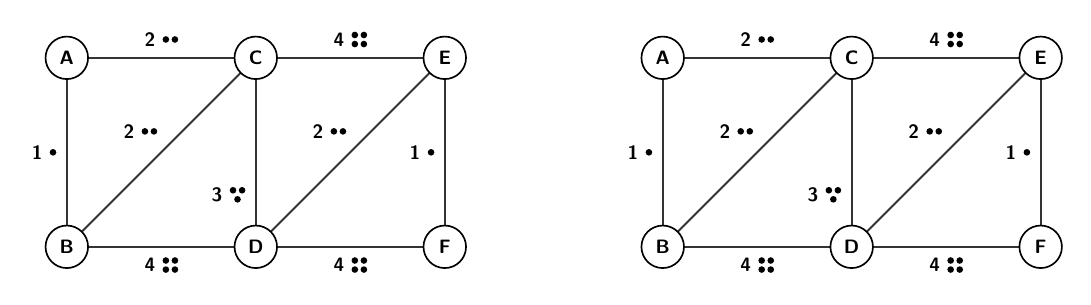
\begin{tikzpicture}[x=1mm,y=1mm]
\draw[line width=0.7pt, black!80] (4.97,27.82) -- (4.97,3.82);
\draw[line width=0.7pt, black!80] (4.97,27.82) -- (28.97,27.82);
\draw[line width=0.7pt, black!80] (4.97,3.82) -- (28.97,27.82);
\draw[line width=0.7pt, black!80] (28.97,27.82) -- (28.97,3.82);
\draw[line width=0.7pt, black!80] (4.97,3.82) -- (28.97,3.82);
\draw[line width=0.7pt, black!80] (28.97,27.82) -- (52.97,27.82);
\draw[line width=0.7pt, black!80] (28.97,3.82) -- (52.97,27.82);
\draw[line width=0.7pt, black!80] (52.97,27.82) -- (52.97,3.82);
\draw[line width=0.7pt, black!80] (28.97,3.82) -- (52.97,3.82);
\fill[white, rounded corners=0.8mm] (0.00,14.32) rectangle (4.15,17.32);
\node[font=\scriptsize\bfseries, inner sep=0] at (1.20,15.82) {1};
\fill (3.22,15.82) circle (0.42mm);
\fill[white, rounded corners=0.8mm] (14.32,28.65) rectangle (19.62,31.65);
\node[font=\scriptsize\bfseries, inner sep=0] at (15.52,30.15) {2};
\fill (17.55,30.15) circle (0.42mm);
\fill (18.70,30.15) circle (0.42mm);
\fill[white, rounded corners=0.8mm] (11.67,16.98) rectangle (16.97,19.98);
\node[font=\scriptsize\bfseries, inner sep=0] at (12.87,18.48) {2};
\fill (14.89,18.48) circle (0.42mm);
\fill (16.04,18.48) circle (0.42mm);
\fill[white, rounded corners=0.8mm] (22.85,8.92) rectangle (28.15,11.92);
\node[font=\scriptsize\bfseries, inner sep=0] at (24.05,10.42) {3};
\fill (26.08,11.00) circle (0.42mm);
\fill (27.23,11.00) circle (0.42mm);
\fill (26.65,9.85) circle (0.42mm);
\fill[white, rounded corners=0.8mm] (14.32,0.00) rectangle (19.62,3.00);
\node[font=\scriptsize\bfseries, inner sep=0] at (15.52,1.50) {4};
\fill (17.55,2.08) circle (0.42mm);
\fill (18.70,2.08) circle (0.42mm);
\fill (17.55,0.93) circle (0.42mm);
\fill (18.70,0.93) circle (0.42mm);
\fill[white, rounded corners=0.8mm] (38.32,28.65) rectangle (43.62,31.65);
\node[font=\scriptsize\bfseries, inner sep=0] at (39.52,30.15) {4};
\fill (41.55,30.72) circle (0.42mm);
\fill (42.70,30.72) circle (0.42mm);
\fill (41.55,29.57) circle (0.42mm);
\fill (42.70,29.57) circle (0.42mm);
\fill[white, rounded corners=0.8mm] (35.67,16.98) rectangle (40.97,19.98);
\node[font=\scriptsize\bfseries, inner sep=0] at (36.87,18.48) {2};
\fill (38.89,18.48) circle (0.42mm);
\fill (40.04,18.48) circle (0.42mm);
\fill[white, rounded corners=0.8mm] (48.00,14.32) rectangle (52.15,17.32);
\node[font=\scriptsize\bfseries, inner sep=0] at (49.20,15.82) {1};
\fill (51.23,15.82) circle (0.42mm);
\fill[white, rounded corners=0.8mm] (38.32,0.00) rectangle (43.62,3.00);
\node[font=\scriptsize\bfseries, inner sep=0] at (39.52,1.50) {4};
\fill (41.55,2.08) circle (0.42mm);
\fill (42.70,2.08) circle (0.42mm);
\fill (41.55,0.93) circle (0.42mm);
\fill (42.70,0.93) circle (0.42mm);
\node[circle, draw, line width=0.6pt, fill=white, minimum size=5.40mm, inner sep=0, font=\scriptsize\bfseries] at (4.97,27.82) {A};
\node[circle, draw, line width=0.6pt, fill=white, minimum size=5.40mm, inner sep=0, font=\scriptsize\bfseries] at (28.97,27.82) {C};
\node[circle, draw, line width=0.6pt, fill=white, minimum size=5.40mm, inner sep=0, font=\scriptsize\bfseries] at (52.97,27.82) {E};
\node[circle, draw, line width=0.6pt, fill=white, minimum size=5.40mm, inner sep=0, font=\scriptsize\bfseries] at (4.97,3.82) {B};
\node[circle, draw, line width=0.6pt, fill=white, minimum size=5.40mm, inner sep=0, font=\scriptsize\bfseries] at (28.97,3.82) {D};
\node[circle, draw, line width=0.6pt, fill=white, minimum size=5.40mm, inner sep=0, font=\scriptsize\bfseries] at (52.97,3.82) {F};
\draw[line width=0.7pt, black!80] (80.65,27.82) -- (80.65,3.82);
\draw[line width=0.7pt, black!80] (80.65,27.82) -- (104.65,27.82);
\draw[line width=0.7pt, black!80] (80.65,3.82) -- (104.65,27.82);
\draw[line width=0.7pt, black!80] (104.65,27.82) -- (104.65,3.82);
\draw[line width=0.7pt, black!80] (80.65,3.82) -- (104.65,3.82);
\draw[line width=0.7pt, black!80] (104.65,27.82) -- (128.65,27.82);
\draw[line width=0.7pt, black!80] (104.65,3.82) -- (128.65,27.82);
\draw[line width=0.7pt, black!80] (128.65,27.82) -- (128.65,3.82);
\draw[line width=0.7pt, black!80] (104.65,3.82) -- (128.65,3.82);
\fill[white, rounded corners=0.8mm] (75.67,14.32) rectangle (79.82,17.32);
\node[font=\scriptsize\bfseries, inner sep=0] at (76.87,15.82) {1};
\fill (78.90,15.82) circle (0.42mm);
\fill[white, rounded corners=0.8mm] (90.00,28.65) rectangle (95.30,31.65);
\node[font=\scriptsize\bfseries, inner sep=0] at (91.20,30.15) {2};
\fill (93.22,30.15) circle (0.42mm);
\fill (94.37,30.15) circle (0.42mm);
\fill[white, rounded corners=0.8mm] (87.34,16.98) rectangle (92.64,19.98);
\node[font=\scriptsize\bfseries, inner sep=0] at (88.54,18.48) {2};
\fill (90.56,18.48) circle (0.42mm);
\fill (91.71,18.48) circle (0.42mm);
\fill[white, rounded corners=0.8mm] (98.52,8.92) rectangle (103.82,11.92);
\node[font=\scriptsize\bfseries, inner sep=0] at (99.72,10.42) {3};
\fill (101.75,11.00) circle (0.42mm);
\fill (102.90,11.00) circle (0.42mm);
\fill (102.32,9.85) circle (0.42mm);
\fill[white, rounded corners=0.8mm] (90.00,0.00) rectangle (95.30,3.00);
\node[font=\scriptsize\bfseries, inner sep=0] at (91.20,1.50) {4};
\fill (93.22,2.08) circle (0.42mm);
\fill (94.37,2.08) circle (0.42mm);
\fill (93.22,0.93) circle (0.42mm);
\fill (94.37,0.93) circle (0.42mm);
\fill[white, rounded corners=0.8mm] (114.00,28.65) rectangle (119.30,31.65);
\node[font=\scriptsize\bfseries, inner sep=0] at (115.20,30.15) {4};
\fill (117.22,30.72) circle (0.42mm);
\fill (118.37,30.72) circle (0.42mm);
\fill (117.22,29.57) circle (0.42mm);
\fill (118.37,29.57) circle (0.42mm);
\fill[white, rounded corners=0.8mm] (111.34,16.98) rectangle (116.64,19.98);
\node[font=\scriptsize\bfseries, inner sep=0] at (112.54,18.48) {2};
\fill (114.56,18.48) circle (0.42mm);
\fill (115.71,18.48) circle (0.42mm);
\fill[white, rounded corners=0.8mm] (123.67,14.32) rectangle (127.82,17.32);
\node[font=\scriptsize\bfseries, inner sep=0] at (124.87,15.82) {1};
\fill (126.90,15.82) circle (0.42mm);
\fill[white, rounded corners=0.8mm] (114.00,0.00) rectangle (119.30,3.00);
\node[font=\scriptsize\bfseries, inner sep=0] at (115.20,1.50) {4};
\fill (117.22,2.08) circle (0.42mm);
\fill (118.37,2.08) circle (0.42mm);
\fill (117.22,0.93) circle (0.42mm);
\fill (118.37,0.93) circle (0.42mm);
\node[circle, draw, line width=0.6pt, fill=white, minimum size=5.40mm, inner sep=0, font=\scriptsize\bfseries] at (80.65,27.82) {A};
\node[circle, draw, line width=0.6pt, fill=white, minimum size=5.40mm, inner sep=0, font=\scriptsize\bfseries] at (104.65,27.82) {C};
\node[circle, draw, line width=0.6pt, fill=white, minimum size=5.40mm, inner sep=0, font=\scriptsize\bfseries] at (128.65,27.82) {E};
\node[circle, draw, line width=0.6pt, fill=white, minimum size=5.40mm, inner sep=0, font=\scriptsize\bfseries] at (80.65,3.82) {B};
\node[circle, draw, line width=0.6pt, fill=white, minimum size=5.40mm, inner sep=0, font=\scriptsize\bfseries] at (104.65,3.82) {D};
\node[circle, draw, line width=0.6pt, fill=white, minimum size=5.40mm, inner sep=0, font=\scriptsize\bfseries] at (128.65,3.82) {F};
\end{tikzpicture}
\end{center}\par

\newpage

\prob{4} Join A, B and C as cheaply as you can, once without the square and once using it. Pay for each in its own pile.

\par\begin{center}
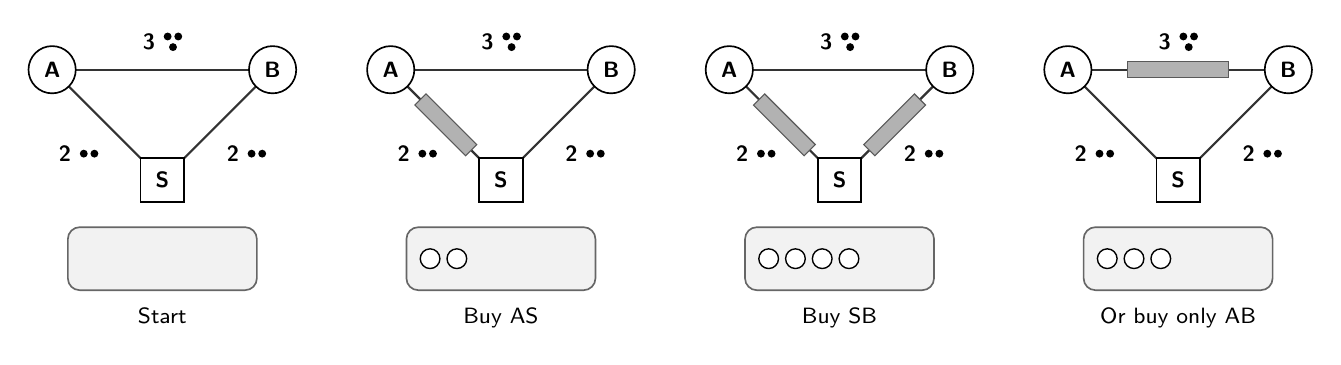
\begin{tikzpicture}[x=1mm,y=1mm]
\draw[line width=0.8pt, black!80] (3.00,29.00) -- (31.00,29.00);
\draw[line width=0.8pt, black!80] (3.00,29.00) -- (17.00,15.00);
\draw[line width=0.8pt, black!80] (17.00,15.00) -- (31.00,29.00);
\fill[white, rounded corners=0.8mm] (13.85,30.74) rectangle (20.15,34.34);
\node[font=\footnotesize\bfseries, inner sep=0] at (15.30,32.54) {3};
\fill (17.67,33.22) circle (0.5mm);
\fill (19.02,33.22) circle (0.5mm);
\fill (18.35,31.87) circle (0.5mm);
\fill[white, rounded corners=0.8mm] (3.19,16.64) rectangle (9.49,20.04);
\node[font=\footnotesize\bfseries, inner sep=0] at (4.64,18.34) {2};
\fill (7.02,18.34) circle (0.5mm);
\fill (8.37,18.34) circle (0.5mm);
\fill[white, rounded corners=0.8mm] (24.51,16.64) rectangle (30.81,20.04);
\node[font=\footnotesize\bfseries, inner sep=0] at (25.96,18.34) {2};
\fill (28.33,18.34) circle (0.5mm);
\fill (29.68,18.34) circle (0.5mm);
\node[circle, draw, line width=0.6pt, fill=white, minimum size=6.00mm, inner sep=0, font=\footnotesize\bfseries] at (3.00,29.00) {A};
\node[circle, draw, line width=0.6pt, fill=white, minimum size=6.00mm, inner sep=0, font=\footnotesize\bfseries] at (31.00,29.00) {B};
\node[rectangle, draw, line width=0.6pt, fill=white, minimum size=5.52mm, inner sep=0, font=\footnotesize\bfseries] at (17.00,15.00) {S};
\draw[black!60, line width=0.6pt, fill=black!5, rounded corners=1.5mm] (5.00,1.00) rectangle (29.00,9.00);
\node[font=\footnotesize, anchor=north, align=center] at (17.00,0.00) {Start};
\draw[line width=0.8pt, black!80] (46.00,29.00) -- (74.00,29.00);
\draw[line width=0.8pt, black!80] (46.00,29.00) -- (60.00,15.00);
\draw[line width=0.8pt, black!80] (60.00,15.00) -- (74.00,29.00);
\filldraw[fill=black!30, draw=black!65, line width=0.4pt] (50.49,25.93) -- (56.93,19.49) -- (55.51,18.07) -- (49.07,24.51) -- cycle;
\fill[white, rounded corners=0.8mm] (56.85,30.74) rectangle (63.15,34.34);
\node[font=\footnotesize\bfseries, inner sep=0] at (58.30,32.54) {3};
\fill (60.68,33.22) circle (0.5mm);
\fill (62.03,33.22) circle (0.5mm);
\fill (61.35,31.87) circle (0.5mm);
\fill[white, rounded corners=0.8mm] (46.19,16.64) rectangle (52.49,20.04);
\node[font=\footnotesize\bfseries, inner sep=0] at (47.64,18.34) {2};
\fill (50.02,18.34) circle (0.5mm);
\fill (51.37,18.34) circle (0.5mm);
\fill[white, rounded corners=0.8mm] (67.51,16.64) rectangle (73.81,20.04);
\node[font=\footnotesize\bfseries, inner sep=0] at (68.96,18.34) {2};
\fill (71.33,18.34) circle (0.5mm);
\fill (72.68,18.34) circle (0.5mm);
\node[circle, draw, line width=0.6pt, fill=white, minimum size=6.00mm, inner sep=0, font=\footnotesize\bfseries] at (46.00,29.00) {A};
\node[circle, draw, line width=0.6pt, fill=white, minimum size=6.00mm, inner sep=0, font=\footnotesize\bfseries] at (74.00,29.00) {B};
\node[rectangle, draw, line width=0.6pt, fill=white, minimum size=5.52mm, inner sep=0, font=\footnotesize\bfseries] at (60.00,15.00) {S};
\draw[black!60, line width=0.6pt, fill=black!5, rounded corners=1.5mm] (48.00,1.00) rectangle (72.00,9.00);
\draw[line width=0.5pt, fill=white] (51.00,5.00) circle (1.25mm);
\draw[line width=0.5pt, fill=white] (54.40,5.00) circle (1.25mm);
\node[font=\footnotesize, anchor=north, align=center] at (60.00,0.00) {Buy AS};
\draw[line width=0.8pt, black!80] (89.00,29.00) -- (117.00,29.00);
\draw[line width=0.8pt, black!80] (89.00,29.00) -- (103.00,15.00);
\draw[line width=0.8pt, black!80] (103.00,15.00) -- (117.00,29.00);
\filldraw[fill=black!30, draw=black!65, line width=0.4pt] (93.49,25.93) -- (99.93,19.49) -- (98.51,18.07) -- (92.07,24.51) -- cycle;
\filldraw[fill=black!30, draw=black!65, line width=0.4pt] (106.07,19.49) -- (112.51,25.93) -- (113.93,24.51) -- (107.49,18.07) -- cycle;
\fill[white, rounded corners=0.8mm] (99.85,30.74) rectangle (106.15,34.34);
\node[font=\footnotesize\bfseries, inner sep=0] at (101.30,32.54) {3};
\fill (103.67,33.22) circle (0.5mm);
\fill (105.03,33.22) circle (0.5mm);
\fill (104.35,31.87) circle (0.5mm);
\fill[white, rounded corners=0.8mm] (89.19,16.64) rectangle (95.49,20.04);
\node[font=\footnotesize\bfseries, inner sep=0] at (90.64,18.34) {2};
\fill (93.02,18.34) circle (0.5mm);
\fill (94.37,18.34) circle (0.5mm);
\fill[white, rounded corners=0.8mm] (110.51,16.64) rectangle (116.81,20.04);
\node[font=\footnotesize\bfseries, inner sep=0] at (111.96,18.34) {2};
\fill (114.33,18.34) circle (0.5mm);
\fill (115.68,18.34) circle (0.5mm);
\node[circle, draw, line width=0.6pt, fill=white, minimum size=6.00mm, inner sep=0, font=\footnotesize\bfseries] at (89.00,29.00) {A};
\node[circle, draw, line width=0.6pt, fill=white, minimum size=6.00mm, inner sep=0, font=\footnotesize\bfseries] at (117.00,29.00) {B};
\node[rectangle, draw, line width=0.6pt, fill=white, minimum size=5.52mm, inner sep=0, font=\footnotesize\bfseries] at (103.00,15.00) {S};
\draw[black!60, line width=0.6pt, fill=black!5, rounded corners=1.5mm] (91.00,1.00) rectangle (115.00,9.00);
\draw[line width=0.5pt, fill=white] (94.00,5.00) circle (1.25mm);
\draw[line width=0.5pt, fill=white] (97.40,5.00) circle (1.25mm);
\draw[line width=0.5pt, fill=white] (100.80,5.00) circle (1.25mm);
\draw[line width=0.5pt, fill=white] (104.20,5.00) circle (1.25mm);
\node[font=\footnotesize, anchor=north, align=center] at (103.00,0.00) {Buy SB};
\draw[line width=0.8pt, black!80] (132.00,29.00) -- (160.00,29.00);
\draw[line width=0.8pt, black!80] (132.00,29.00) -- (146.00,15.00);
\draw[line width=0.8pt, black!80] (146.00,15.00) -- (160.00,29.00);
\filldraw[fill=black!30, draw=black!65, line width=0.4pt] (139.56,30.00) -- (152.44,30.00) -- (152.44,28.00) -- (139.56,28.00) -- cycle;
\fill[white, rounded corners=0.8mm] (142.85,30.74) rectangle (149.15,34.34);
\node[font=\footnotesize\bfseries, inner sep=0] at (144.30,32.54) {3};
\fill (146.67,33.22) circle (0.5mm);
\fill (148.02,33.22) circle (0.5mm);
\fill (147.35,31.87) circle (0.5mm);
\fill[white, rounded corners=0.8mm] (132.19,16.64) rectangle (138.49,20.04);
\node[font=\footnotesize\bfseries, inner sep=0] at (133.64,18.34) {2};
\fill (136.02,18.34) circle (0.5mm);
\fill (137.37,18.34) circle (0.5mm);
\fill[white, rounded corners=0.8mm] (153.51,16.64) rectangle (159.81,20.04);
\node[font=\footnotesize\bfseries, inner sep=0] at (154.96,18.34) {2};
\fill (157.33,18.34) circle (0.5mm);
\fill (158.68,18.34) circle (0.5mm);
\node[circle, draw, line width=0.6pt, fill=white, minimum size=6.00mm, inner sep=0, font=\footnotesize\bfseries] at (132.00,29.00) {A};
\node[circle, draw, line width=0.6pt, fill=white, minimum size=6.00mm, inner sep=0, font=\footnotesize\bfseries] at (160.00,29.00) {B};
\node[rectangle, draw, line width=0.6pt, fill=white, minimum size=5.52mm, inner sep=0, font=\footnotesize\bfseries] at (146.00,15.00) {S};
\draw[black!60, line width=0.6pt, fill=black!5, rounded corners=1.5mm] (134.00,1.00) rectangle (158.00,9.00);
\draw[line width=0.5pt, fill=white] (137.00,5.00) circle (1.25mm);
\draw[line width=0.5pt, fill=white] (140.40,5.00) circle (1.25mm);
\draw[line width=0.5pt, fill=white] (143.80,5.00) circle (1.25mm);
\node[font=\footnotesize, anchor=north, align=center] at (146.00,0.00) {Or buy only AB};
\end{tikzpicture}
\end{center}\par

\par\begin{center}
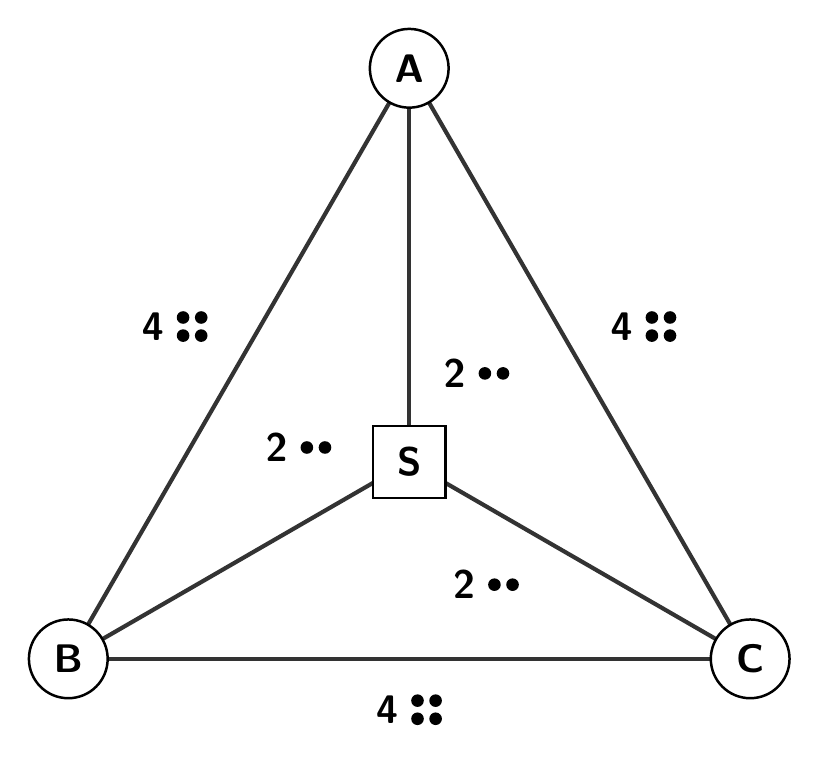
\begin{tikzpicture}[x=1mm,y=1mm]
\draw[line width=1.5pt, black!80] (48.30,84.46) -- (5.00,9.46);
\draw[line width=1.5pt, black!80] (5.00,9.46) -- (91.60,9.46);
\draw[line width=1.5pt, black!80] (48.30,84.46) -- (91.60,9.46);
\draw[line width=1.5pt, black!80] (48.30,34.46) -- (48.30,84.46);
\draw[line width=1.5pt, black!80] (48.30,34.46) -- (5.00,9.46);
\draw[line width=1.5pt, black!80] (48.30,34.46) -- (91.60,9.46);
\fill[white, rounded corners=0.8mm] (13.43,48.66) rectangle (23.63,54.66);
\node[font=\Large\bfseries, inner sep=0] at (15.73,51.66) {4};
\fill (19.58,52.81) circle (0.8mm);
\fill (21.88,52.81) circle (0.8mm);
\fill (19.58,50.51) circle (0.8mm);
\fill (21.88,50.51) circle (0.8mm);
\fill[white, rounded corners=0.8mm] (43.20,0.00) rectangle (53.40,6.00);
\node[font=\Large\bfseries, inner sep=0] at (45.50,3.00) {4};
\fill (49.35,4.15) circle (0.8mm);
\fill (51.65,4.15) circle (0.8mm);
\fill (49.35,1.85) circle (0.8mm);
\fill (51.65,1.85) circle (0.8mm);
\fill[white, rounded corners=0.8mm] (72.97,48.66) rectangle (83.17,54.66);
\node[font=\Large\bfseries, inner sep=0] at (75.27,51.66) {4};
\fill (79.12,52.81) circle (0.8mm);
\fill (81.42,52.81) circle (0.8mm);
\fill (79.12,50.51) circle (0.8mm);
\fill (81.42,50.51) circle (0.8mm);
\fill[white, rounded corners=0.8mm] (51.76,42.71) rectangle (61.96,48.71);
\node[font=\Large\bfseries, inner sep=0] at (54.06,45.71) {2};
\fill (57.91,45.71) circle (0.8mm);
\fill (60.21,45.71) circle (0.8mm);
\fill[white, rounded corners=0.8mm] (29.15,33.30) rectangle (39.35,39.30);
\node[font=\Large\bfseries, inner sep=0] at (31.45,36.30) {2};
\fill (35.30,36.30) circle (0.8mm);
\fill (37.60,36.30) circle (0.8mm);
\fill[white, rounded corners=0.8mm] (52.97,15.88) rectangle (63.17,21.88);
\node[font=\Large\bfseries, inner sep=0] at (55.27,18.88) {2};
\fill (59.12,18.88) circle (0.8mm);
\fill (61.42,18.88) circle (0.8mm);
\node[circle, draw, line width=0.9pt, fill=white, minimum size=10.00mm, inner sep=0, font=\Large\bfseries] at (48.30,84.46) {A};
\node[circle, draw, line width=0.9pt, fill=white, minimum size=10.00mm, inner sep=0, font=\Large\bfseries] at (5.00,9.46) {B};
\node[circle, draw, line width=0.9pt, fill=white, minimum size=10.00mm, inner sep=0, font=\Large\bfseries] at (91.60,9.46) {C};
\node[rectangle, draw, line width=0.9pt, fill=white, minimum size=9.20mm, inner sep=0, font=\Large\bfseries] at (48.30,34.46) {S};
\end{tikzpicture}
\end{center}\par

\vspace{6mm}
\begin{center}
without the square \raisebox{-3mm}{\tikz[x=1mm,y=1mm]{\draw[black!60, line width=0.6pt] (0,0) rectangle (18,10);}}
\hspace{18mm}
using the square \raisebox{-3mm}{\tikz[x=1mm,y=1mm]{\draw[black!60, line width=0.6pt] (0,0) rectangle (18,10);}}
\end{center}

\newpage

\prob{5} On each map, join the circles as cheaply as you can, once without the square and once using it. Does the square save counters?

\par\begin{center}
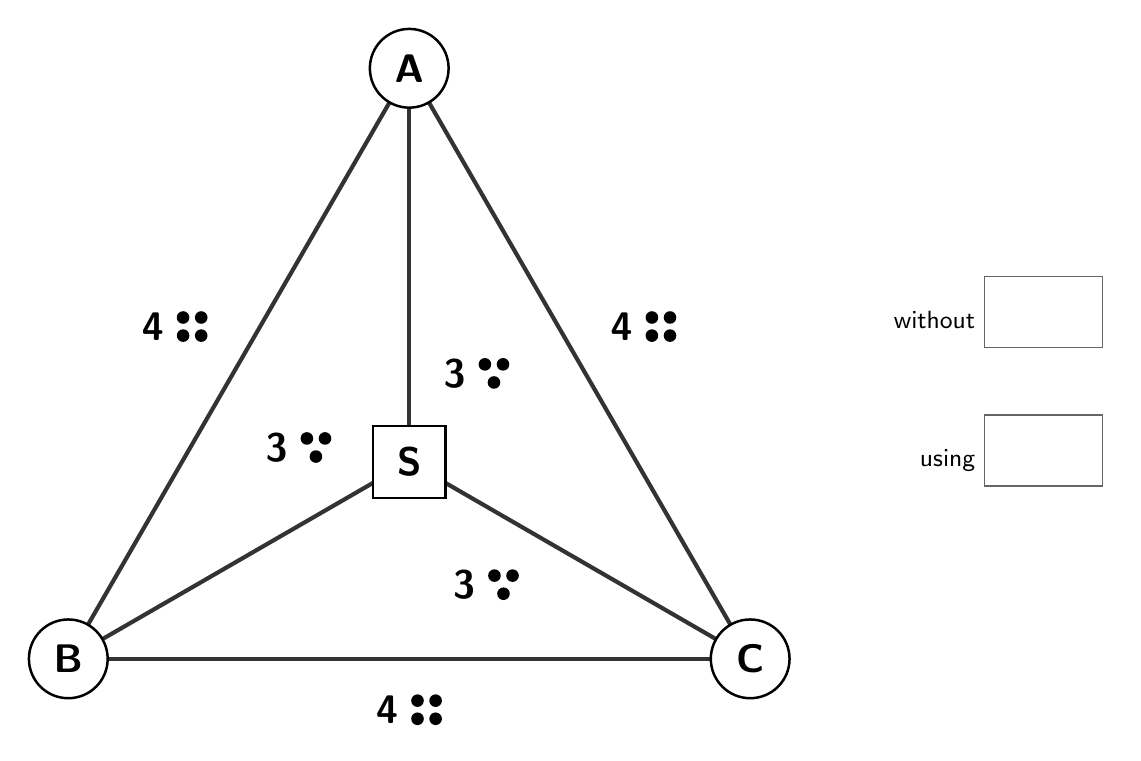
\begin{tikzpicture}[x=1mm,y=1mm]
\draw[line width=1.5pt, black!80] (48.30,84.46) -- (5.00,9.46);
\draw[line width=1.5pt, black!80] (5.00,9.46) -- (91.60,9.46);
\draw[line width=1.5pt, black!80] (48.30,84.46) -- (91.60,9.46);
\draw[line width=1.5pt, black!80] (48.30,34.46) -- (48.30,84.46);
\draw[line width=1.5pt, black!80] (48.30,34.46) -- (5.00,9.46);
\draw[line width=1.5pt, black!80] (48.30,34.46) -- (91.60,9.46);
\fill[white, rounded corners=0.8mm] (13.43,48.66) rectangle (23.63,54.66);
\node[font=\Large\bfseries, inner sep=0] at (15.73,51.66) {4};
\fill (19.58,52.81) circle (0.8mm);
\fill (21.88,52.81) circle (0.8mm);
\fill (19.58,50.51) circle (0.8mm);
\fill (21.88,50.51) circle (0.8mm);
\fill[white, rounded corners=0.8mm] (43.20,0.00) rectangle (53.40,6.00);
\node[font=\Large\bfseries, inner sep=0] at (45.50,3.00) {4};
\fill (49.35,4.15) circle (0.8mm);
\fill (51.65,4.15) circle (0.8mm);
\fill (49.35,1.85) circle (0.8mm);
\fill (51.65,1.85) circle (0.8mm);
\fill[white, rounded corners=0.8mm] (72.97,48.66) rectangle (83.17,54.66);
\node[font=\Large\bfseries, inner sep=0] at (75.27,51.66) {4};
\fill (79.12,52.81) circle (0.8mm);
\fill (81.42,52.81) circle (0.8mm);
\fill (79.12,50.51) circle (0.8mm);
\fill (81.42,50.51) circle (0.8mm);
\fill[white, rounded corners=0.8mm] (51.76,42.71) rectangle (61.96,48.71);
\node[font=\Large\bfseries, inner sep=0] at (54.06,45.71) {3};
\fill (57.91,46.86) circle (0.8mm);
\fill (60.21,46.86) circle (0.8mm);
\fill (59.06,44.56) circle (0.8mm);
\fill[white, rounded corners=0.8mm] (29.15,33.30) rectangle (39.35,39.30);
\node[font=\Large\bfseries, inner sep=0] at (31.45,36.30) {3};
\fill (35.30,37.45) circle (0.8mm);
\fill (37.60,37.45) circle (0.8mm);
\fill (36.45,35.15) circle (0.8mm);
\fill[white, rounded corners=0.8mm] (52.97,15.88) rectangle (63.17,21.88);
\node[font=\Large\bfseries, inner sep=0] at (55.27,18.88) {3};
\fill (59.12,20.03) circle (0.8mm);
\fill (61.42,20.03) circle (0.8mm);
\fill (60.27,17.73) circle (0.8mm);
\node[circle, draw, line width=0.9pt, fill=white, minimum size=10.00mm, inner sep=0, font=\Large\bfseries] at (48.30,84.46) {A};
\node[circle, draw, line width=0.9pt, fill=white, minimum size=10.00mm, inner sep=0, font=\Large\bfseries] at (5.00,9.46) {B};
\node[circle, draw, line width=0.9pt, fill=white, minimum size=10.00mm, inner sep=0, font=\Large\bfseries] at (91.60,9.46) {C};
\node[rectangle, draw, line width=0.9pt, fill=white, minimum size=9.20mm, inner sep=0, font=\Large\bfseries] at (48.30,34.46) {S};
\node[anchor=west, font=\small, align=right] at (108.60,44.73) {without \raisebox{-2.5mm}{\tikz[x=1mm,y=1mm]{\draw[black!60, line width=0.6pt] (0,0) rectangle (15,9);}}\\[8mm] using \raisebox{-2.5mm}{\tikz[x=1mm,y=1mm]{\draw[black!60, line width=0.6pt] (0,0) rectangle (15,9);}}};
\end{tikzpicture}
\end{center}\par

\vspace{2mm}
\par\begin{center}
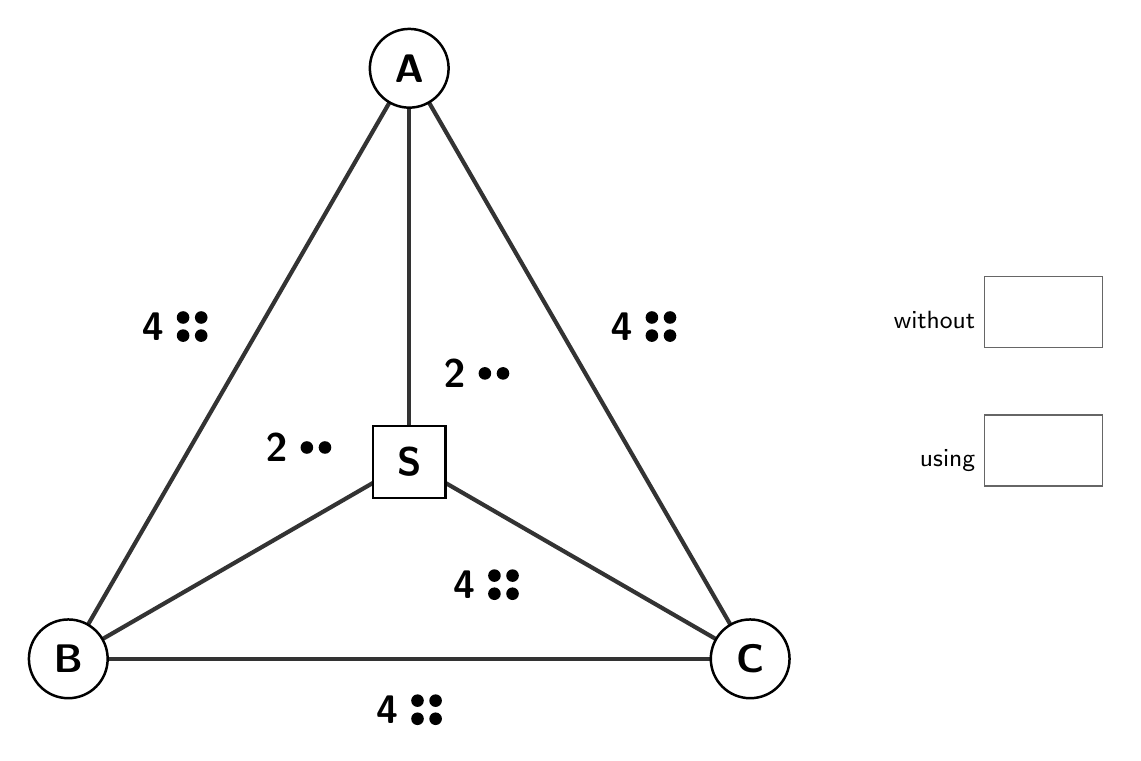
\begin{tikzpicture}[x=1mm,y=1mm]
\draw[line width=1.5pt, black!80] (48.30,84.46) -- (5.00,9.46);
\draw[line width=1.5pt, black!80] (5.00,9.46) -- (91.60,9.46);
\draw[line width=1.5pt, black!80] (48.30,84.46) -- (91.60,9.46);
\draw[line width=1.5pt, black!80] (48.30,34.46) -- (48.30,84.46);
\draw[line width=1.5pt, black!80] (48.30,34.46) -- (5.00,9.46);
\draw[line width=1.5pt, black!80] (48.30,34.46) -- (91.60,9.46);
\fill[white, rounded corners=0.8mm] (13.43,48.66) rectangle (23.63,54.66);
\node[font=\Large\bfseries, inner sep=0] at (15.73,51.66) {4};
\fill (19.58,52.81) circle (0.8mm);
\fill (21.88,52.81) circle (0.8mm);
\fill (19.58,50.51) circle (0.8mm);
\fill (21.88,50.51) circle (0.8mm);
\fill[white, rounded corners=0.8mm] (43.20,0.00) rectangle (53.40,6.00);
\node[font=\Large\bfseries, inner sep=0] at (45.50,3.00) {4};
\fill (49.35,4.15) circle (0.8mm);
\fill (51.65,4.15) circle (0.8mm);
\fill (49.35,1.85) circle (0.8mm);
\fill (51.65,1.85) circle (0.8mm);
\fill[white, rounded corners=0.8mm] (72.97,48.66) rectangle (83.17,54.66);
\node[font=\Large\bfseries, inner sep=0] at (75.27,51.66) {4};
\fill (79.12,52.81) circle (0.8mm);
\fill (81.42,52.81) circle (0.8mm);
\fill (79.12,50.51) circle (0.8mm);
\fill (81.42,50.51) circle (0.8mm);
\fill[white, rounded corners=0.8mm] (51.76,42.71) rectangle (61.96,48.71);
\node[font=\Large\bfseries, inner sep=0] at (54.06,45.71) {2};
\fill (57.91,45.71) circle (0.8mm);
\fill (60.21,45.71) circle (0.8mm);
\fill[white, rounded corners=0.8mm] (29.15,33.30) rectangle (39.35,39.30);
\node[font=\Large\bfseries, inner sep=0] at (31.45,36.30) {2};
\fill (35.30,36.30) circle (0.8mm);
\fill (37.60,36.30) circle (0.8mm);
\fill[white, rounded corners=0.8mm] (52.97,15.88) rectangle (63.17,21.88);
\node[font=\Large\bfseries, inner sep=0] at (55.27,18.88) {4};
\fill (59.12,20.03) circle (0.8mm);
\fill (61.42,20.03) circle (0.8mm);
\fill (59.12,17.73) circle (0.8mm);
\fill (61.42,17.73) circle (0.8mm);
\node[circle, draw, line width=0.9pt, fill=white, minimum size=10.00mm, inner sep=0, font=\Large\bfseries] at (48.30,84.46) {A};
\node[circle, draw, line width=0.9pt, fill=white, minimum size=10.00mm, inner sep=0, font=\Large\bfseries] at (5.00,9.46) {B};
\node[circle, draw, line width=0.9pt, fill=white, minimum size=10.00mm, inner sep=0, font=\Large\bfseries] at (91.60,9.46) {C};
\node[rectangle, draw, line width=0.9pt, fill=white, minimum size=9.20mm, inner sep=0, font=\Large\bfseries] at (48.30,34.46) {S};
\node[anchor=west, font=\small, align=right] at (108.60,44.73) {without \raisebox{-2.5mm}{\tikz[x=1mm,y=1mm]{\draw[black!60, line width=0.6pt] (0,0) rectangle (15,9);}}\\[8mm] using \raisebox{-2.5mm}{\tikz[x=1mm,y=1mm]{\draw[black!60, line width=0.6pt] (0,0) rectangle (15,9);}}};
\end{tikzpicture}
\end{center}\par

\vspace{2mm}
\newpage

\prob{6} Join the circles as cheaply as you can, once without the square and once using it. Does the square save counters?

\par\begin{center}
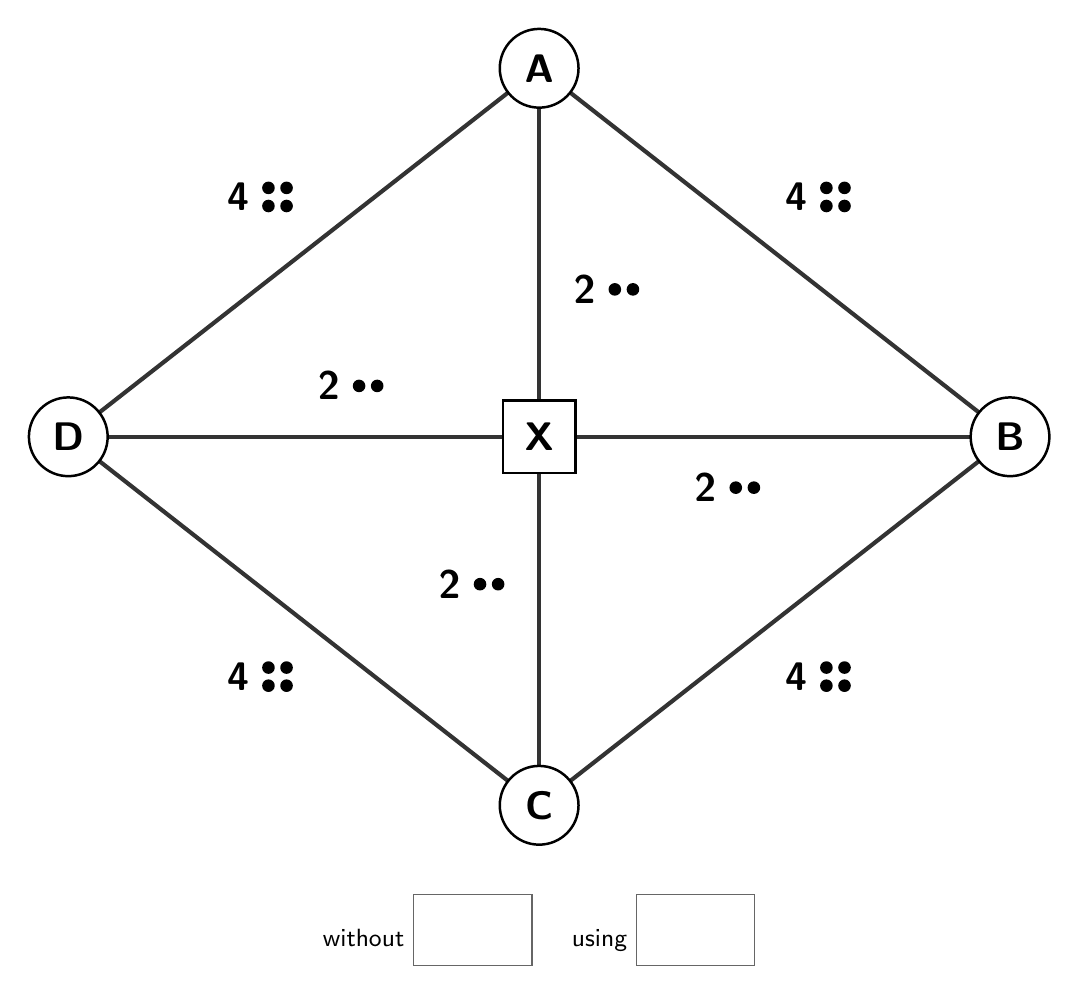
\begin{tikzpicture}[x=1mm,y=1mm]
\draw[line width=1.5pt, black!80] (64.80,112.60) -- (124.60,65.80);
\draw[line width=1.5pt, black!80] (124.60,65.80) -- (64.80,19.00);
\draw[line width=1.5pt, black!80] (64.80,19.00) -- (5.00,65.80);
\draw[line width=1.5pt, black!80] (5.00,65.80) -- (64.80,112.60);
\draw[line width=1.5pt, black!80] (64.80,65.80) -- (64.80,112.60);
\draw[line width=1.5pt, black!80] (64.80,65.80) -- (124.60,65.80);
\draw[line width=1.5pt, black!80] (64.80,65.80) -- (64.80,19.00);
\draw[line width=1.5pt, black!80] (64.80,65.80) -- (5.00,65.80);
\fill[white, rounded corners=0.8mm] (95.13,93.26) rectangle (105.33,99.26);
\node[font=\Large\bfseries, inner sep=0] at (97.43,96.26) {4};
\fill (101.28,97.41) circle (0.8mm);
\fill (103.58,97.41) circle (0.8mm);
\fill (101.28,95.11) circle (0.8mm);
\fill (103.58,95.11) circle (0.8mm);
\fill[white, rounded corners=0.8mm] (95.13,32.34) rectangle (105.33,38.34);
\node[font=\Large\bfseries, inner sep=0] at (97.43,35.34) {4};
\fill (101.28,36.49) circle (0.8mm);
\fill (103.58,36.49) circle (0.8mm);
\fill (101.28,34.19) circle (0.8mm);
\fill (103.58,34.19) circle (0.8mm);
\fill[white, rounded corners=0.8mm] (24.27,32.34) rectangle (34.47,38.34);
\node[font=\Large\bfseries, inner sep=0] at (26.57,35.34) {4};
\fill (30.42,36.49) circle (0.8mm);
\fill (32.72,36.49) circle (0.8mm);
\fill (30.42,34.19) circle (0.8mm);
\fill (32.72,34.19) circle (0.8mm);
\fill[white, rounded corners=0.8mm] (24.27,93.26) rectangle (34.47,99.26);
\node[font=\Large\bfseries, inner sep=0] at (26.57,96.26) {4};
\fill (30.42,97.41) circle (0.8mm);
\fill (32.72,97.41) circle (0.8mm);
\fill (30.42,95.11) circle (0.8mm);
\fill (32.72,95.11) circle (0.8mm);
\fill[white, rounded corners=0.8mm] (68.26,81.52) rectangle (78.46,87.52);
\node[font=\Large\bfseries, inner sep=0] at (70.56,84.52) {2};
\fill (74.41,84.52) circle (0.8mm);
\fill (76.71,84.52) circle (0.8mm);
\fill[white, rounded corners=0.8mm] (83.62,56.34) rectangle (93.82,62.34);
\node[font=\Large\bfseries, inner sep=0] at (85.92,59.34) {2};
\fill (89.77,59.34) circle (0.8mm);
\fill (92.07,59.34) circle (0.8mm);
\fill[white, rounded corners=0.8mm] (51.14,44.08) rectangle (61.34,50.08);
\node[font=\Large\bfseries, inner sep=0] at (53.44,47.08) {2};
\fill (57.29,47.08) circle (0.8mm);
\fill (59.59,47.08) circle (0.8mm);
\fill[white, rounded corners=0.8mm] (35.78,69.26) rectangle (45.98,75.26);
\node[font=\Large\bfseries, inner sep=0] at (38.08,72.26) {2};
\fill (41.93,72.26) circle (0.8mm);
\fill (44.23,72.26) circle (0.8mm);
\node[circle, draw, line width=0.9pt, fill=white, minimum size=10.00mm, inner sep=0, font=\Large\bfseries] at (64.80,112.60) {A};
\node[circle, draw, line width=0.9pt, fill=white, minimum size=10.00mm, inner sep=0, font=\Large\bfseries] at (124.60,65.80) {B};
\node[circle, draw, line width=0.9pt, fill=white, minimum size=10.00mm, inner sep=0, font=\Large\bfseries] at (64.80,19.00) {C};
\node[circle, draw, line width=0.9pt, fill=white, minimum size=10.00mm, inner sep=0, font=\Large\bfseries] at (5.00,65.80) {D};
\node[rectangle, draw, line width=0.9pt, fill=white, minimum size=9.20mm, inner sep=0, font=\Large\bfseries] at (64.80,65.80) {X};
\node[anchor=north, font=\small] at (64.80,9) {without \raisebox{-2.5mm}{\tikz[x=1mm,y=1mm]{\draw[black!60, line width=0.6pt] (0,0) rectangle (15,9);}}\hspace{5mm}using \raisebox{-2.5mm}{\tikz[x=1mm,y=1mm]{\draw[black!60, line width=0.6pt] (0,0) rectangle (15,9);}}};
\end{tikzpicture}
\end{center}\par

\vspace{1mm}
\newpage

\prob{7} Join A, B, C and D as cheaply as you can.

\par\begin{center}
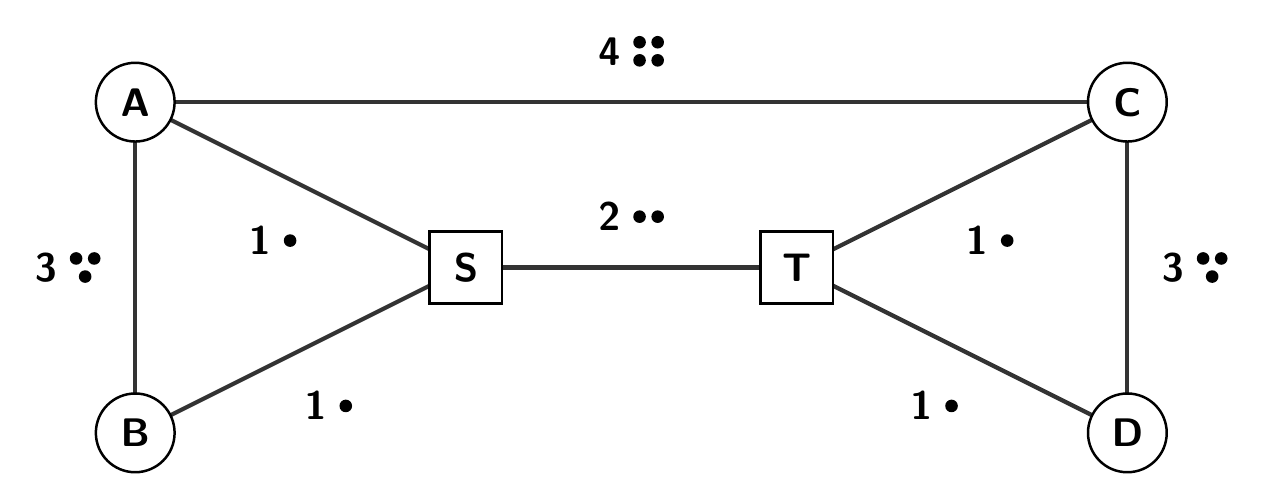
\begin{tikzpicture}[x=1mm,y=1mm]
\draw[line width=1.5pt, black!80] (13.66,47.00) -- (55.66,26.00);
\draw[line width=1.5pt, black!80] (13.66,5.00) -- (55.66,26.00);
\draw[line width=1.5pt, black!80] (55.66,26.00) -- (97.66,26.00);
\draw[line width=1.5pt, black!80] (97.66,26.00) -- (139.66,47.00);
\draw[line width=1.5pt, black!80] (97.66,26.00) -- (139.66,5.00);
\draw[line width=1.5pt, black!80] (13.66,47.00) -- (13.66,5.00);
\draw[line width=1.5pt, black!80] (139.66,47.00) -- (139.66,5.00);
\draw[line width=1.5pt, black!80] (13.66,47.00) -- (139.66,47.00);
\fill[white, rounded corners=0.8mm] (27.18,26.42) rectangle (35.08,32.42);
\node[font=\Large\bfseries, inner sep=0] at (29.48,29.42) {1};
\fill (33.33,29.42) circle (0.8mm);
\fill[white, rounded corners=0.8mm] (34.25,5.42) rectangle (42.15,11.42);
\node[font=\Large\bfseries, inner sep=0] at (36.55,8.42) {1};
\fill (40.40,8.42) circle (0.8mm);
\fill[white, rounded corners=0.8mm] (71.56,29.46) rectangle (81.76,35.46);
\node[font=\Large\bfseries, inner sep=0] at (73.86,32.46) {2};
\fill (77.71,32.46) circle (0.8mm);
\fill (80.01,32.46) circle (0.8mm);
\fill[white, rounded corners=0.8mm] (118.25,26.42) rectangle (126.15,32.42);
\node[font=\Large\bfseries, inner sep=0] at (120.55,29.42) {1};
\fill (124.40,29.42) circle (0.8mm);
\fill[white, rounded corners=0.8mm] (111.18,5.42) rectangle (119.08,11.42);
\node[font=\Large\bfseries, inner sep=0] at (113.48,8.42) {1};
\fill (117.33,8.42) circle (0.8mm);
\fill[white, rounded corners=0.8mm] (0.00,23.00) rectangle (10.20,29.00);
\node[font=\Large\bfseries, inner sep=0] at (2.30,26.00) {3};
\fill (6.15,27.15) circle (0.8mm);
\fill (8.45,27.15) circle (0.8mm);
\fill (7.30,24.85) circle (0.8mm);
\fill[white, rounded corners=0.8mm] (143.13,23.00) rectangle (153.33,29.00);
\node[font=\Large\bfseries, inner sep=0] at (145.43,26.00) {3};
\fill (149.28,27.15) circle (0.8mm);
\fill (151.58,27.15) circle (0.8mm);
\fill (150.43,24.85) circle (0.8mm);
\fill[white, rounded corners=0.8mm] (71.56,50.46) rectangle (81.76,56.46);
\node[font=\Large\bfseries, inner sep=0] at (73.86,53.46) {4};
\fill (77.71,54.61) circle (0.8mm);
\fill (80.01,54.61) circle (0.8mm);
\fill (77.71,52.31) circle (0.8mm);
\fill (80.01,52.31) circle (0.8mm);
\node[circle, draw, line width=0.9pt, fill=white, minimum size=10.00mm, inner sep=0, font=\Large\bfseries] at (13.66,47.00) {A};
\node[circle, draw, line width=0.9pt, fill=white, minimum size=10.00mm, inner sep=0, font=\Large\bfseries] at (13.66,5.00) {B};
\node[rectangle, draw, line width=0.9pt, fill=white, minimum size=9.20mm, inner sep=0, font=\Large\bfseries] at (55.66,26.00) {S};
\node[rectangle, draw, line width=0.9pt, fill=white, minimum size=9.20mm, inner sep=0, font=\Large\bfseries] at (97.66,26.00) {T};
\node[circle, draw, line width=0.9pt, fill=white, minimum size=10.00mm, inner sep=0, font=\Large\bfseries] at (139.66,47.00) {C};
\node[circle, draw, line width=0.9pt, fill=white, minimum size=10.00mm, inner sep=0, font=\Large\bfseries] at (139.66,5.00) {D};
\end{tikzpicture}
\end{center}\par

\vspace{1mm}
\par\begin{center}
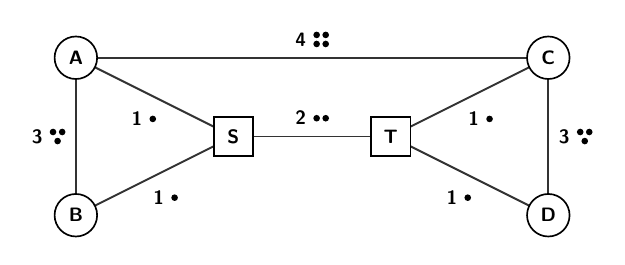
\begin{tikzpicture}[x=1mm,y=1mm]
\draw[line width=0.7pt, black!80] (6.12,22.70) -- (26.12,12.70);
\draw[line width=0.7pt, black!80] (6.12,2.70) -- (26.12,12.70);
\draw[line width=0.7pt, black!80] (26.12,12.70) -- (46.12,12.70);
\draw[line width=0.7pt, black!80] (46.12,12.70) -- (66.12,22.70);
\draw[line width=0.7pt, black!80] (46.12,12.70) -- (66.12,2.70);
\draw[line width=0.7pt, black!80] (6.12,22.70) -- (6.12,2.70);
\draw[line width=0.7pt, black!80] (66.12,22.70) -- (66.12,2.70);
\draw[line width=0.7pt, black!80] (6.12,22.70) -- (66.12,22.70);
\fill[white, rounded corners=0.8mm] (12.67,13.43) rectangle (16.82,16.43);
\node[font=\scriptsize\bfseries, inner sep=0] at (13.87,14.93) {1};
\fill (15.89,14.93) circle (0.42mm);
\fill[white, rounded corners=0.8mm] (15.43,3.43) rectangle (19.58,6.43);
\node[font=\scriptsize\bfseries, inner sep=0] at (16.63,4.93) {1};
\fill (18.66,4.93) circle (0.42mm);
\fill[white, rounded corners=0.8mm] (33.47,13.52) rectangle (38.77,16.52);
\node[font=\scriptsize\bfseries, inner sep=0] at (34.67,15.02) {2};
\fill (36.70,15.02) circle (0.42mm);
\fill (37.85,15.02) circle (0.42mm);
\fill[white, rounded corners=0.8mm] (55.43,13.43) rectangle (59.58,16.43);
\node[font=\scriptsize\bfseries, inner sep=0] at (56.63,14.93) {1};
\fill (58.66,14.93) circle (0.42mm);
\fill[white, rounded corners=0.8mm] (52.67,3.43) rectangle (56.82,6.43);
\node[font=\scriptsize\bfseries, inner sep=0] at (53.87,4.93) {1};
\fill (55.89,4.93) circle (0.42mm);
\fill[white, rounded corners=0.8mm] (0.00,11.20) rectangle (5.30,14.20);
\node[font=\scriptsize\bfseries, inner sep=0] at (1.20,12.70) {3};
\fill (3.22,13.27) circle (0.42mm);
\fill (4.38,13.27) circle (0.42mm);
\fill (3.80,12.12) circle (0.42mm);
\fill[white, rounded corners=0.8mm] (66.95,11.20) rectangle (72.25,14.20);
\node[font=\scriptsize\bfseries, inner sep=0] at (68.15,12.70) {3};
\fill (70.17,13.27) circle (0.42mm);
\fill (71.32,13.27) circle (0.42mm);
\fill (70.75,12.12) circle (0.42mm);
\fill[white, rounded corners=0.8mm] (33.47,23.52) rectangle (38.77,26.52);
\node[font=\scriptsize\bfseries, inner sep=0] at (34.67,25.02) {4};
\fill (36.70,25.60) circle (0.42mm);
\fill (37.85,25.60) circle (0.42mm);
\fill (36.70,24.45) circle (0.42mm);
\fill (37.85,24.45) circle (0.42mm);
\node[circle, draw, line width=0.6pt, fill=white, minimum size=5.40mm, inner sep=0, font=\scriptsize\bfseries] at (6.12,22.70) {A};
\node[circle, draw, line width=0.6pt, fill=white, minimum size=5.40mm, inner sep=0, font=\scriptsize\bfseries] at (6.12,2.70) {B};
\node[rectangle, draw, line width=0.6pt, fill=white, minimum size=4.97mm, inner sep=0, font=\scriptsize\bfseries] at (26.12,12.70) {S};
\node[rectangle, draw, line width=0.6pt, fill=white, minimum size=4.97mm, inner sep=0, font=\scriptsize\bfseries] at (46.12,12.70) {T};
\node[circle, draw, line width=0.6pt, fill=white, minimum size=5.40mm, inner sep=0, font=\scriptsize\bfseries] at (66.12,22.70) {C};
\node[circle, draw, line width=0.6pt, fill=white, minimum size=5.40mm, inner sep=0, font=\scriptsize\bfseries] at (66.12,2.70) {D};
\end{tikzpicture}
\end{center}\par

\vspace{5mm}
\prob{8} Draw dots on the links to the square so that joining A, B and C as cheaply as you can costs the same using the square as without it.

\par\begin{center}
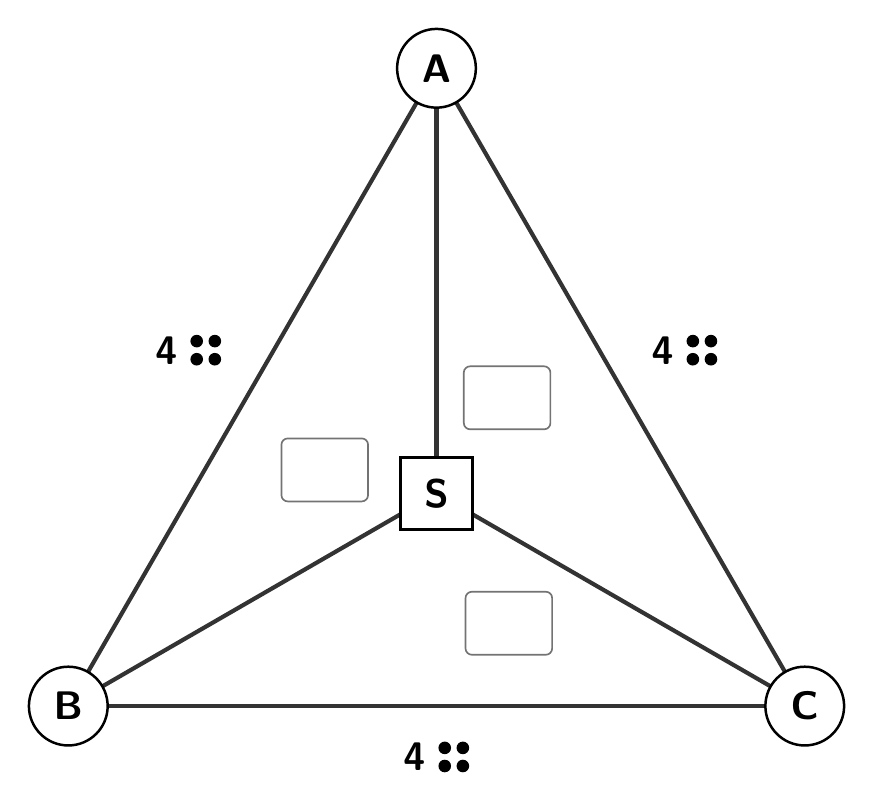
\begin{tikzpicture}[x=1mm,y=1mm]
\draw[line width=1.5pt, black!80] (51.76,90.46) -- (5.00,9.46);
\draw[line width=1.5pt, black!80] (5.00,9.46) -- (98.53,9.46);
\draw[line width=1.5pt, black!80] (51.76,90.46) -- (98.53,9.46);
\draw[line width=1.5pt, black!80] (51.76,36.46) -- (51.76,90.46);
\draw[line width=1.5pt, black!80] (51.76,36.46) -- (5.00,9.46);
\draw[line width=1.5pt, black!80] (51.76,36.46) -- (98.53,9.46);
\fill[white, rounded corners=0.8mm] (15.16,51.66) rectangle (25.36,57.66);
\node[font=\Large\bfseries, inner sep=0] at (17.46,54.66) {4};
\fill (21.31,55.81) circle (0.8mm);
\fill (23.61,55.81) circle (0.8mm);
\fill (21.31,53.51) circle (0.8mm);
\fill (23.61,53.51) circle (0.8mm);
\fill[white, rounded corners=0.8mm] (46.66,0.00) rectangle (56.86,6.00);
\node[font=\Large\bfseries, inner sep=0] at (48.96,3.00) {4};
\fill (52.81,4.15) circle (0.8mm);
\fill (55.11,4.15) circle (0.8mm);
\fill (52.81,1.85) circle (0.8mm);
\fill (55.11,1.85) circle (0.8mm);
\fill[white, rounded corners=0.8mm] (78.17,51.66) rectangle (88.37,57.66);
\node[font=\Large\bfseries, inner sep=0] at (80.47,54.66) {4};
\fill (84.32,55.81) circle (0.8mm);
\fill (86.62,55.81) circle (0.8mm);
\fill (84.32,53.51) circle (0.8mm);
\fill (86.62,53.51) circle (0.8mm);
\draw[black!55, line width=0.6pt, fill=white, rounded corners=0.8mm] (55.23,44.61) rectangle (66.23,52.61);
\draw[black!55, line width=0.6pt, fill=white, rounded corners=0.8mm] (32.07,35.45) rectangle (43.07,43.45);
\draw[black!55, line width=0.6pt, fill=white, rounded corners=0.8mm] (55.45,15.98) rectangle (66.45,23.98);
\node[circle, draw, line width=0.9pt, fill=white, minimum size=10.00mm, inner sep=0, font=\Large\bfseries] at (51.76,90.46) {A};
\node[circle, draw, line width=0.9pt, fill=white, minimum size=10.00mm, inner sep=0, font=\Large\bfseries] at (5.00,9.46) {B};
\node[circle, draw, line width=0.9pt, fill=white, minimum size=10.00mm, inner sep=0, font=\Large\bfseries] at (98.53,9.46) {C};
\node[rectangle, draw, line width=0.9pt, fill=white, minimum size=9.20mm, inner sep=0, font=\Large\bfseries] at (51.76,36.46) {S};
\end{tikzpicture}
\end{center}\par

\end{document}
